\chapter{Deep Learning}

Deep Learning (DL) is a subfield of Neural Networks (NN) which in turn is a subfield of Machine Learning (ML) which again is a subfield of Artificial Intelligence (AI). Figure~\ref{fig:MLOverview} shows a Neural Network relevant taxonomy of AI. There are many advantages of ML over more traditional statistical methods as often found e.g. in statistical learning. Some of these advantages are that ML does not require any hypothesis and deep understanding of the underlying data. While statistical learning is mostly about inference (deducing properties of an underlying probability distribution, sampled from a larger population), ML is mostly about predictions in supervised, unsupervised and semi-supervised learning. It also does not operate on assumptions like normality, multicollinearity and homoscedasticity, etc.. Statistical Learning operates on much smaller datasets with only a few attributes and therefore is less fit for problems with millions of possible and possibly unknown attributes and data samples. Machine Learning excels at identifying patterns in large datasets through many iterations and thus being able to predict or classify previously unseen data.

Traditional Machine Learning approaches were based on very specific feature extractions that needed to be found/created manually and could take months to fine tune. The biggest downside was that the features often were not generalizable and were very domain specific. Even looking at the same object from different angles or from different photographs often needed additional fine-tuning of existing features or creating new ones. Some of the feature extraction algorithms include Scale Invariant Feature Transform (SIFT), Histogram Oriented Gradient (HOG), Local Binary Pattern (LBP) and others. Learning algorithms that are applied on these features are e.g.: Support Vector Machines (SVM), Random Forest (RF), Principal Component Analysis (PCA), Kernel PCA (KPCA), Linear Decrement Analysis (LDA), Fisher Decrement Analysis (FDA) and many more. New Machine Learning methods are able to automatically learn feature representations which is much less labor-intensive and often very surprising as well because features are learned that don't intuitively make sense but nonetheless perform quite well. Special caution should be exercised in not trusting the models too much. Sometimes, the model performs really but actually has learned something useless that correlates with the labels provided but has no causality.\\


\begin{figure}[!h]
  \centering
  \caption{Partial taxonomy of Artificial Inteligence~\cite{alom2018history}}
  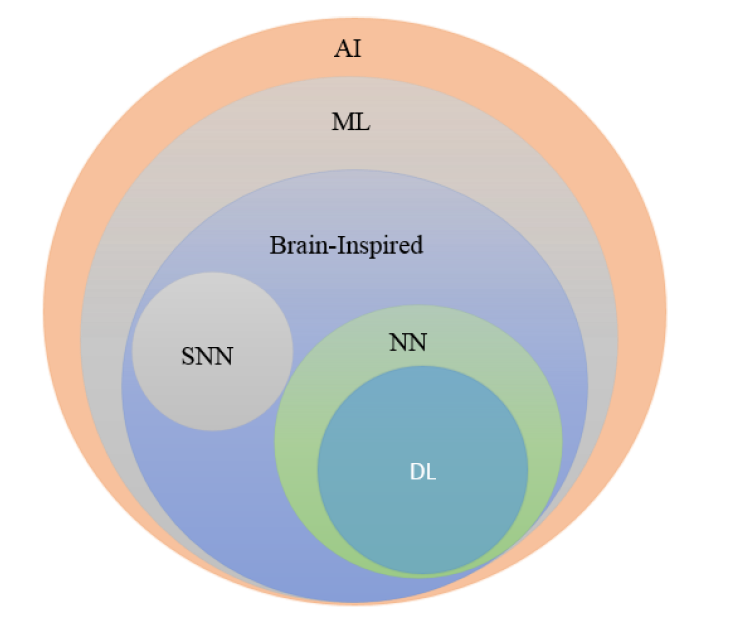
\includegraphics[scale=0.4]{chapter3/MLOverview}
  \label{fig:MLOverview}
\end{figure}

\section{Artificial Neural Network}

An Artificial Neural Network (ANN) tries to mimic the behavior of the human brain to some extent. The analogy of the artificial neuron helps to understand the parallels between information processing in biological and artificial neurons, but it is only an analogy and therefore should be used very cautiously. There are many more differences than similarities like different neuron types, diverse electrophysiological make-up of neurons, neurotransmitters and receptor blockers, plasticity~\cite{brunel2014single, london2005dendritic}. The human brain is still a huge mystery in most aspects. Nonetheless, the abstract notion of a neuron is visually very appealing and useful. Figure~\ref{fig:Neurons} shows on the left side a biological neuron with all its relevant parts and the mathematical representation of it on the right side. The biological neuron receives its inputs from other neurons through its dendrites (through many different neurotransmitters in the synapses). If a certain energy threshold is reached in the cell body from all its incoming dendrites, it transmits the information along the axon to other neurons. The axon branches out towards its end and may reach several different neurons and the process continues. Learning is believed to happen when the sensitivity of the synapses changes and new pathways are formed through branching the axon and connecting to new axons or making the current pathways stronger.


\begin{figure}[!h]
  \centering
  \caption{A biological neuron on the left versus the mathematical representation of a neuron on the right. The mathematical represenation shows the exact implementation how neurons are used in CNNs~\cite{cs231neuralnetworks}.}
  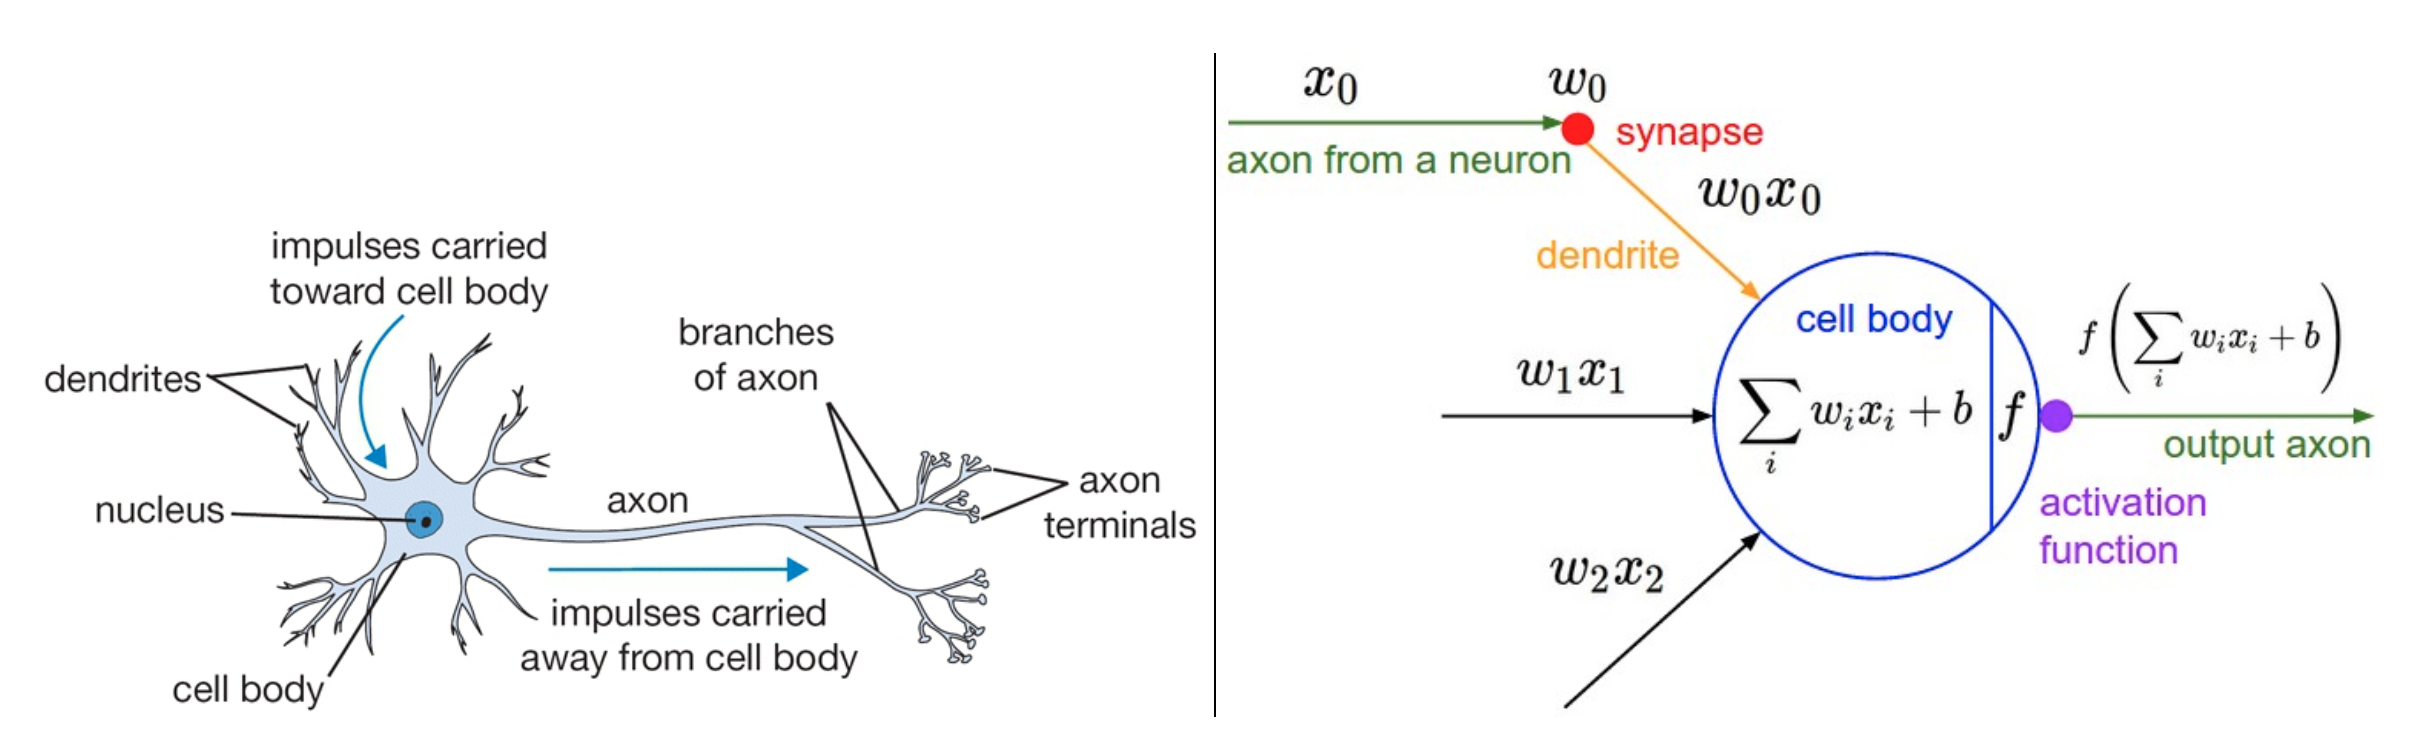
\includegraphics[scale=0.35]{chapter3/Neurons}
  \label{fig:Neurons}
\end{figure}

\quad

This is indeed similar to how an artificial neuron processes its received information and how it passes the information forward to the next layers. An artificial neuron receives inputs (e.g. $x_0$) from other neurons in prior layers and applies a weight matrix (e.g. $w_0$) and a bias (e.g. $b$) on it. The weights and the bias can be compared to the strength of the synapses in the biological neuron and these can be changed through learning. Actually, that is what happens during backpropagation explained later on. The weights are adjusted in order to classify the input more accurately. In the cell body of the mathematical representation a dot product between the inputs and the weights is performed and a bias is added to it ($w_i x_i + b$). In the end a certain activation function is applied to it. This activation function needs to be non-linear because otherwise all the matrix computations of different neurons could be collapsed into one linear computation and no learning would take place. Instead, just a linear regression would be achieved.
Traditionally a sigmoid function has been used for the activation function since it takes any real number as input and outputs numbers between 0 and 1. That is a very intuitive non-linearity function to work with but has some disadvantages when backpropagating the loss function and adjusting the parameters in the weight matrices.  During backpropagation, the loss is computed according to some loss function and then back propagated through all layers and units. During that process, the partial derivatives of the loss function are computed with respect to the input variables (e.g. $x_i^j$) of that specific unit. In the used notation the superscript denotes the layer whereas the subscript denotes the unit within that specific layer. These derivatives are then multiplied by a learning rate alpha and added to the current weights. This process of changing the weights towards an optimal loss is called learning and happens through many iterations (also called epochs). In Figure~\ref{fig:SigmoidTanh} two activation functions, the sigmoid and the tanh, are shown. Since the partial derivatives are crucial in learning - the steeper the derivation the bigger the change in weights - the disadvantages of both non-linearities are clearly visible towards the borders. If the function moves mostly horizontally, the first derivation will be near 0 thus learning happens very slow. The tanh has a steeper function around the center (leading to a bigger first derivative and thus faster learning) but still has the same problem towards the borders.\\


\begin{figure}[!h]
  \centering
  \caption{The sigmoid non-linearity takes in any real number and outputs a number in the range [0,1], wheras the tanh non-linearity takes the same input but outputs a number in the range of [-1,1]. Both lead to very slow learning if the input is not centered around 0~\cite{cs231neuralnetworks}.}
  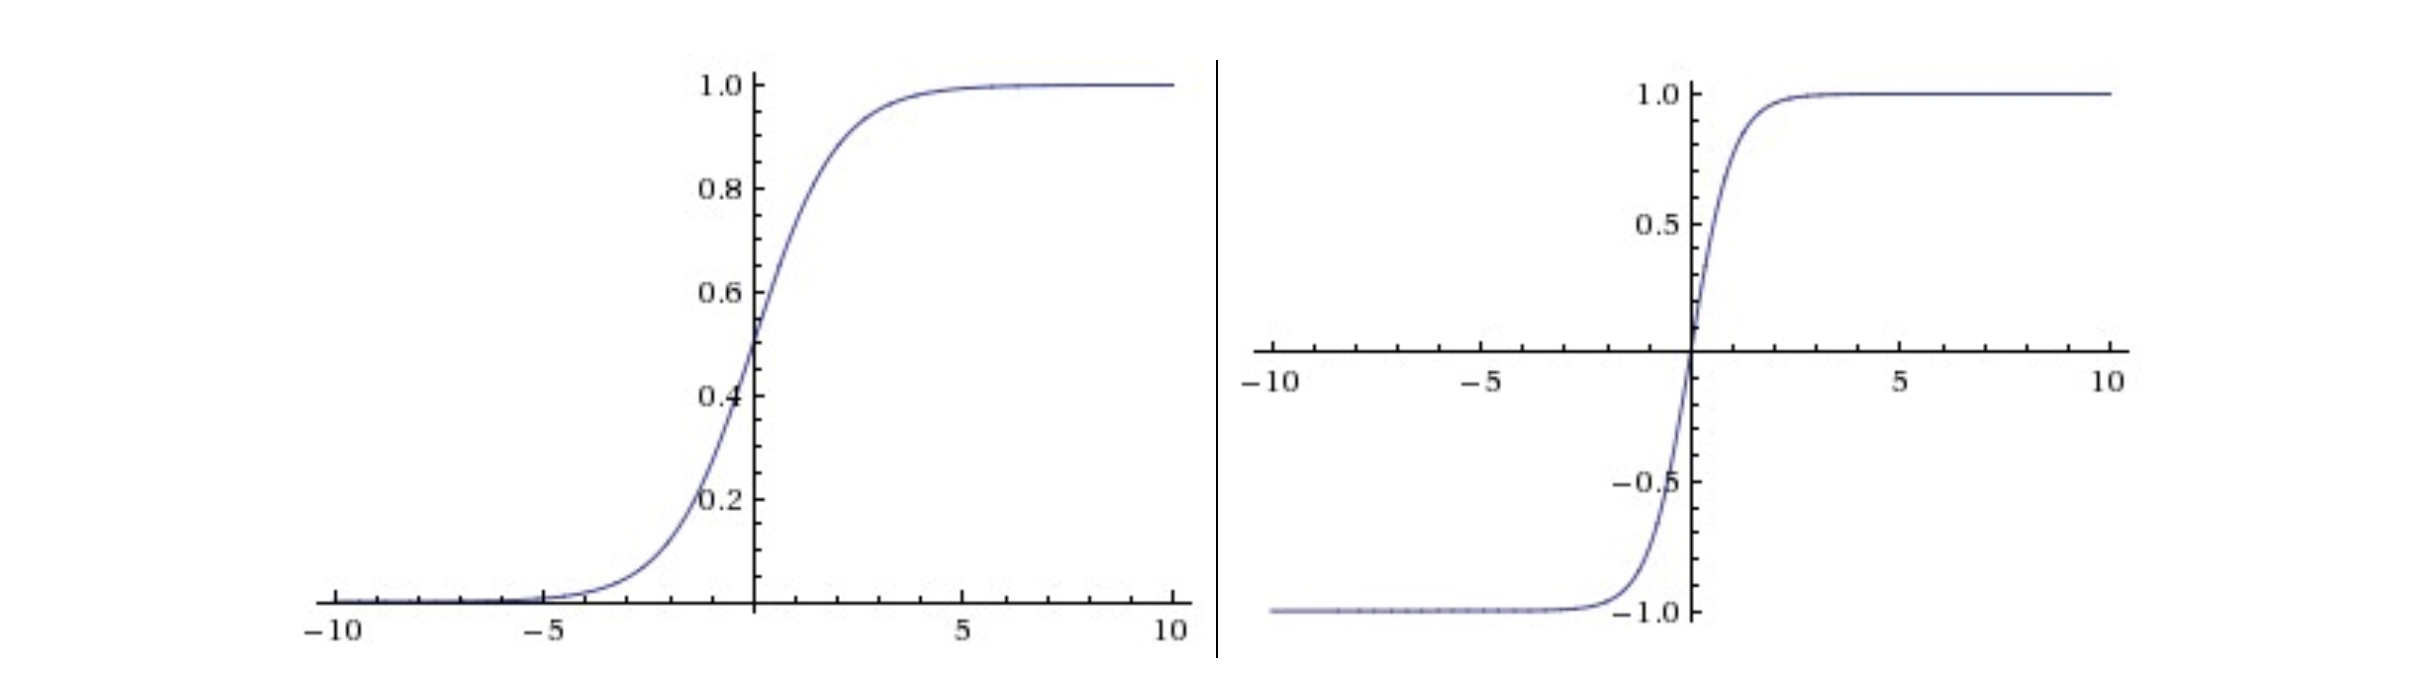
\includegraphics[scale=0.4]{chapter3/SigmoidTanh}
  \label{fig:SigmoidTanh}
\end{figure}

\quad

For the above-mentioned reasons, the sigmoid non-linearity is not used anymore except in the last layer and only if the task is a binary classification. For that special case, the sigmoid is still a valid function. As an alternative, the Rectified Linear Unit (ReLU) is used. It is very simple, fast to compute and easy to back-propagate since the derivatives are 0 or a fixed value. In order to omit the deactivation of units, which happens when the input values are smaller than 0, a leaky ReLU can be used. Both non-linearities can be seen in Figure~\ref{fig:ReLU}.\\


\begin{figure}[!h]
  \centering
  \caption{Rectified Liner Unit on the right side. It deactivates the units when their input values are negative. A Leaky ReLU has not this disadvantage and never deactivates the units~\cite{reinventingNN}.}
  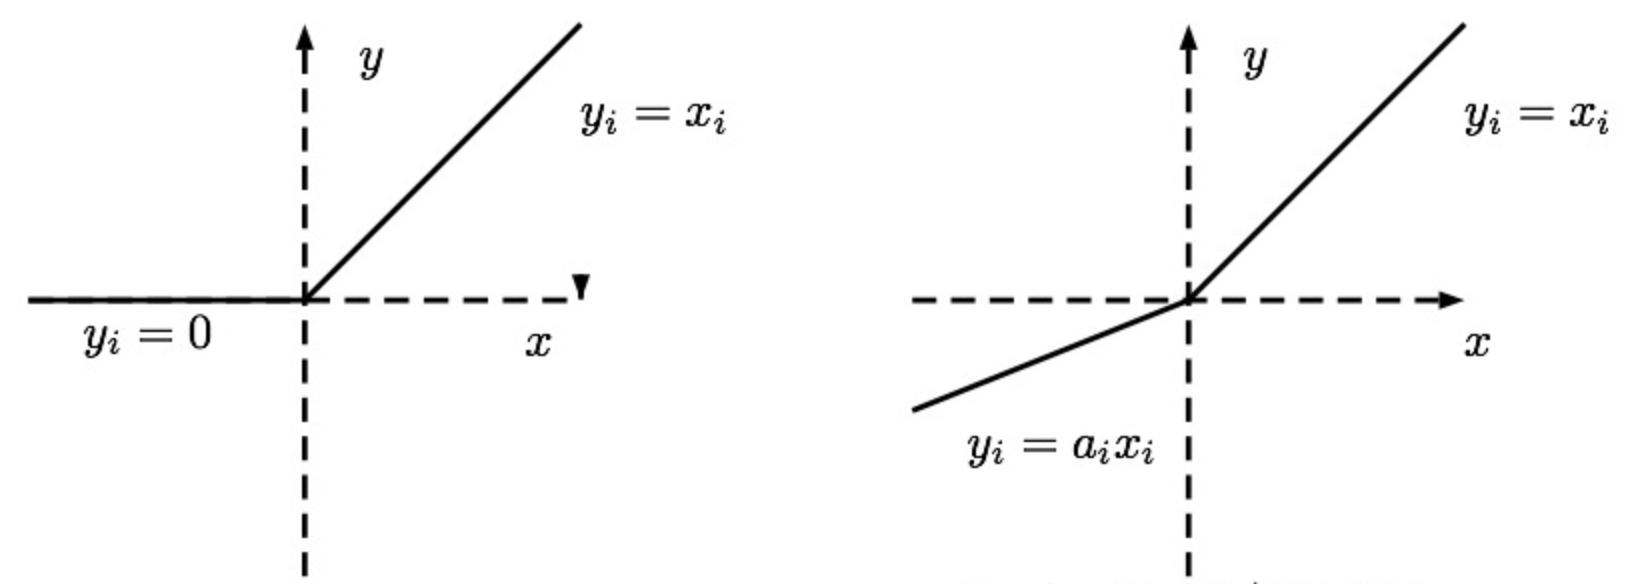
\includegraphics[scale=0.4]{chapter3/ReLU}
  \label{fig:ReLU}
\end{figure}

\quad

The components of an Artificial Neural Network (ANN) are the units (neurons) organized in an acyclic graph. All units that are reached from the input layer by the same amount of hops are organized into distinct layers denoted with a superscript index. These units are not connected to each other but to the next layer as shown in Figure~\ref{fig:MLP}. As the name suggests cycles are not allowed since the forward and backward pass would not be well defined anymore. Another big difference to the human brain where acyclic connections are possible and very common. Neuroscience even shows us that the human brain is fundamentally cyclic~\cite{goodale1992separate}. Very recent research tries to implement these feedback loops into neural nets~\cite{caswell2016loopy}, but that is beyond the scope of this thesis. Subsequent layers within the ANN are fully connected with each other, meaning every unit connects to every unit in the next layer. These networks are called Multi-Layer Perceptrons (MLP). One of the problems with MLP's is that the fully-connected nature of this architecture increases the number of parameters exponentially. To illustrate this problem an RGB image of 256 by 256 pixels can be considered. It has an input size of 196'608 (256x256x3) pixel values. If this is multiplied with the next layer having only 1000 hidden units the result is already 196'608'000 distinct pixel values meaning there are roughly 197 million parameters to be held in memory and updated with every iteration just for the first layer. One pixel value is in the range of 0 to 255 which means 8 bits or 1 byte. Current image compression formats like png or jpeg are able to compress this information, but witout compression as full blown array values, that would mean 197 MB of memory only for a small image in memory. Every unit in this layer would have 196'608 weights which is absolutely wasteful since so many parameters with rather simple images lead to severe overfitting. Another big disadvantage of this kind of fully connected image recognition is the fact that there is no spatial encoding in the network. It is very nicely observed with the MNIST dataset where images (28x28 pixels) of handwritten digits are provided~\cite{MNISTdatabase}. The MLP learns that the image contains a certain number only by learning which pixels need to be black in order to match the previously seen labels. That leads to a near-perfect recognition of the centered digit 2 but if the digit is moved to the border (different distribution of black pixels) the MLP is not able to recognize the digit anymore.\\


\begin{figure}[!h]
  \centering
  \caption{Two multi-layer perceptrons where each layer is fully connected with the subsequent layer leading to an exponential growth of connections and weights. On the left side a 2-layer network is shown, on the right side a 3-layer network. The first layer is not counted towards the layer count~\cite{cs231nconvolution}.}
  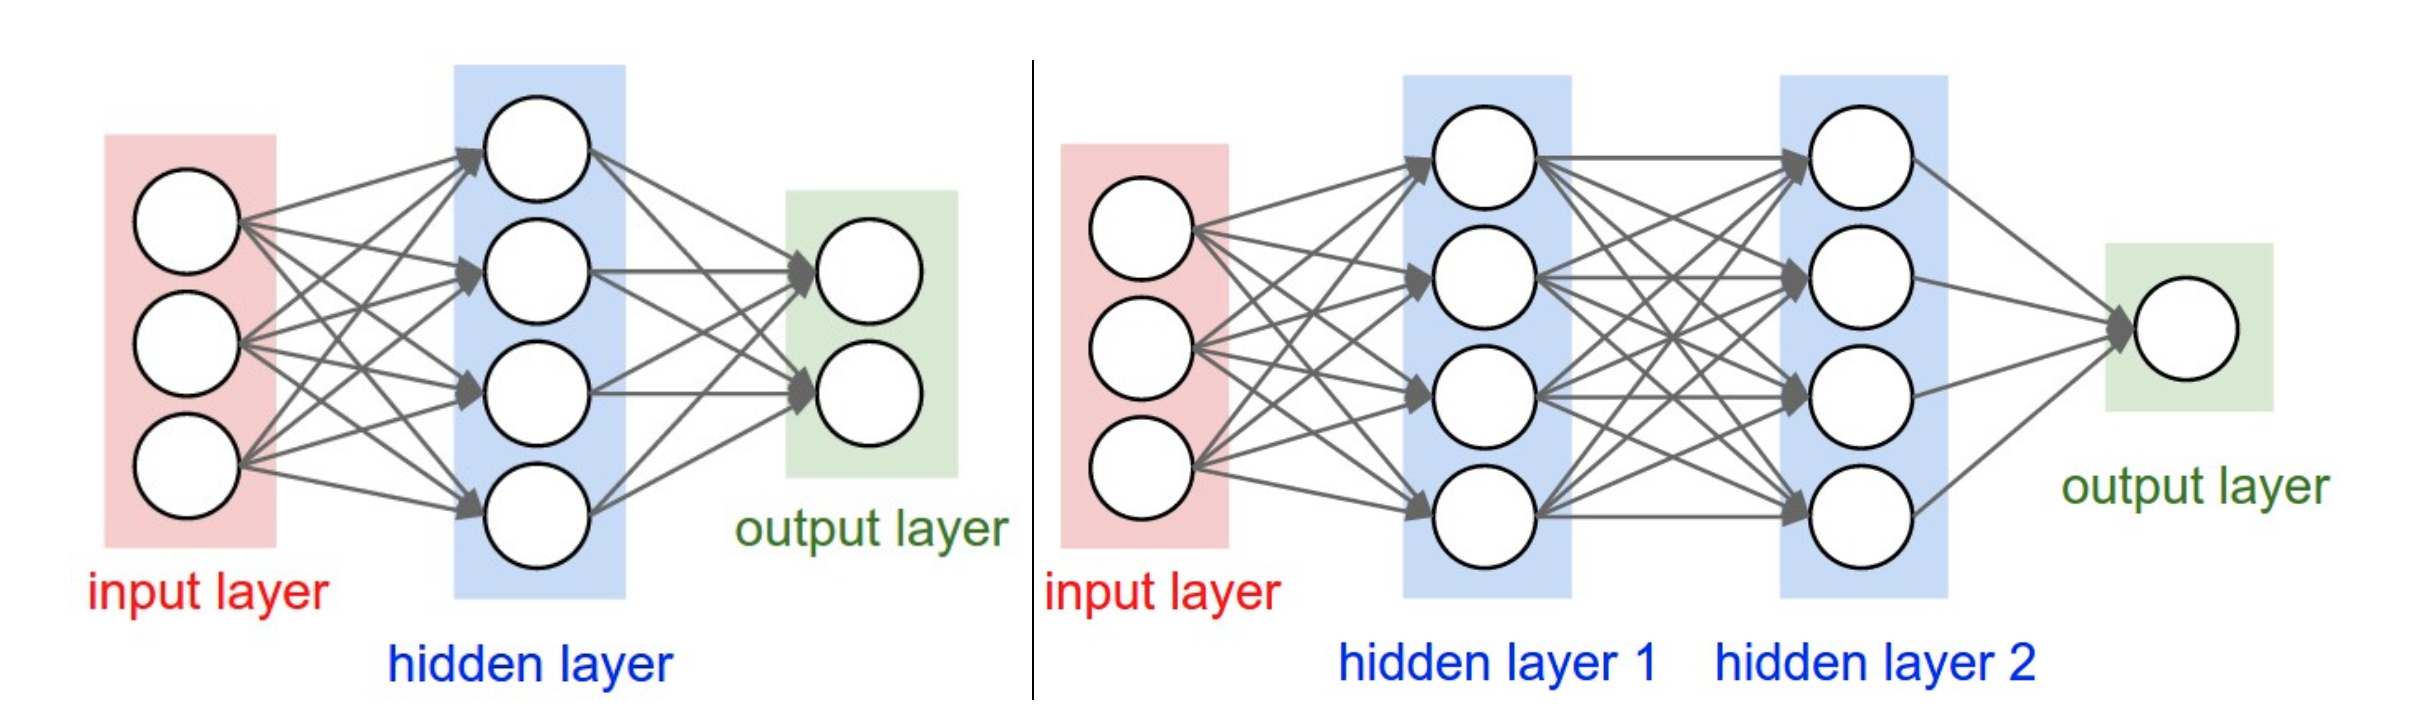
\includegraphics[scale=0.36]{chapter3/MLP}
  \label{fig:MLP}
\end{figure}

\quad

There are several deep learning networks like Unsupervised Pretrained Networks (UPNs), Convolutional Neural Networks (CNNs), and Recurrent Neural Networks (RNNs)~\cite{typesOfANN, deepLearningAdam}. UPNs consist of several subcategories like Deep Belief Networks (DBNs) that use unsupervised pre-training to learn higher-level feature representations or Generative Adversarial Networks (GANs) that can create new images from existing ones. CNNs have proven themselves to be a superior fit on pure image recognition task since they apply small convolutions to extract spatial characteristic patterns from the image that are used for classification. RNNs are useful for anything that comes in a temporal sequence like a video or a text input feed. In order to translate a sentence from one language into another not only the current word is of importance  but the context in which it is used, meaning what came previously and what comes after the word.\\


\section{ImageNet Large Scale Visual Recognition Challenge (ILSVRC)}

The ImageNet Large Scale Visual Recognition Challenge (ILSVRC) has become the standard benchmark for object recognition and is held annually since 2010~\cite{imagenet}. It has borrowed many concepts from the PASCAL VOC 2010 dataset but increased the amount of data drastically, from 19'737 images in PASCAL VOC 2010 with 20 object classes to 1'461'406 images and 1000 object classes in ILSVRC 2010~\cite{everingham2010pascal, russakovsky2015imagenet}. ILSVRC consists of two components: the dataset that is publicly available and consists of over 1.2 million annotated, high-resolution images (train set), and the annual competition with its workshops. The test set, ranging from 100'000 to 150'000 images, is also released but without the labels. Participants are able to train their models on the datasets and annotate the images in the test set. The annotated test set is then sent to the evaluation server where the overall score is computed~\cite{russakovsky2015imagenet}. With the ImageNet Challenge, there are two main competitions namely object detection for 200 fully labeled categories and object localization for 1000 categories (binary label for presence or absence of an object). For the object localization, there are two main metrics, the top-1 error rate and the top-5 error rate. The top-1 error rate shows the percentage for which the correct class was not correctly predicted (only the first top label is observed). The top-5 error rate shows the percentage of test examples for which the correct label was not in the top 5 predicted classes. Since ILSVRC 2015 new competition tasks are added like object detection from video or scene classification, but they are less relevant for this thesis~\cite{imagenet2015}. Before ILSVRC many datasets were available for training models like Caltech 101~\cite{fei2007learning} with 101 object classes and Caltech 256~\cite{griffin2007caltech} with 256 object classes. Both were tiny at best when compared to the ImageNet dataset. TinyImages~\cite{torralba200880} is a huge dataset with 80 million images but the images are only 32 by 32 pixels which makes them low-resolution. Also, the images are not manually verified thus leading to many incorrect labels.

In 2010 and 2011 the winners used traditional machine learning approaches like HOG, LBP and FV for dense grid descriptors and SVM for feature application with other more specialized methods. In 2012, AlexNet (a 5-layer CNN) beat all competitors by a large margin. It was the beginning of a new chapter in machine learning, namely the chapter of Convolutional Neural Networks and Deep Learning in the field of computer vision. Since then, only CNNs are winning the ILSVRC with ResNet surpassing human level accuracy in 2015~\cite{he2016deep}. Human level accuracy was obtained when Andrej Karpathy took it on and labeled 1'500 test images after having trained on 500 validation images. It took him a few days and he reached an astonishing 5.1\% top-5 error rate while other scientists giving it a try reached around 12\% error rate~\cite{humanlevel2014}.

It is also worth noting that ImageNet is the most widely used dataset for transfer learning. Pre-trained weights for most of the current state-of-the-art architectures are widely available on the internet and can be downloaded. In transfer learning a specific architecture is trained for weeks on a dataset, then the weights of all filters in all layers are made publicly available. All feature mappings are therefore already present and only need to be fine-tuned, which reduces the time needed to train a model drastically. All evaluation in Chapter 5 related to transfer learning is based on weights pre-trained on ImageNet.\\


\section{Convolutional Neural Networks}

Convolutional Neural Networks (CNNs) are a subset of Neural Networks so they still share most of the components like an input layer, hidden layers with their units, possibly a fully connected layer at the end of the architecture, a loss function, forward and backward propagation. The big difference is that CNNs explicitly expect images as input whereas a Neural Network expects nothing in particular, just a single vector of data. Knowing that the input is an image, the architecture can be changed accordingly, leading to spatial awareness through convolutions and vastly reduced parameters. Spatial awareness means that additionally to knowing the value of one pixel (in the first layer) a convolution encodes the values of neighboring pixels as well, thus giving some representation of an area of nearby pixels. Figure~\ref{fig:Convolution} shows a simple convolution step where a filter of 5x5x3 is applied over the image. The filters depth (3rd dimension) is always equal to the input volume's depth. Since the image is RGB encoded the depth of the image is 3, so are the filters in the first layer. The filter, sometimes also called kernel, is then convolved across the whole image and a dot product is computed at every position. This gives an activation map, seen in blue on the right side in Figure~\ref{fig:Convolution}. Each filter that is convolved across the image produces a different activation map that usually is slightly smaller than the original input but becomes deeper with every additional layer since more filters are added. The goal of the learning process is to learn different filters, that represent specific characteristics of the image and lead to a correct classification, thus reducing the loss. As mentioned at the beginning of this chapter, a huge advantage of modern machine learning methods is that the feature maps are learned automatically by the architecture. The best filters, leading to a minimal loss, will be found without the need of manually crafting specific feature maps like HOG. That saves time and leads to much more generalizable models.\\


\begin{figure}[!h]
  \centering
  \caption{A 5x5x3 kernel is convolved over the 32x32x3 image generating a 28x28x1 output volume. The number of kernels used gives the depth of the output volume~\cite{cs231nconvolution}.}
  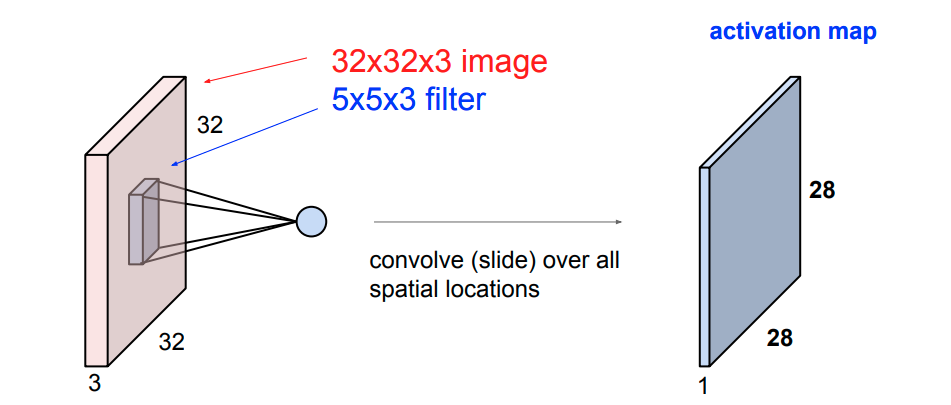
\includegraphics[scale=0.35]{chapter3/Convolution}
  \label{fig:Convolution}
\end{figure}

\quad

Instead of connecting all the neurons of one layer to all the neurons of the subsequent layer leading to an exponential growth of parameters, now each neuron is only connected to a local region of the input. The 5x5x3 filter shown in Figure~\ref{fig:Convolution} has a receptive filed of 5x5. The depth of the filter must always be equal to the depth of the input volume (input image in the first layer), and the number of filters used in a specific layer represents the new depth of the output volume.

In order to build a CNN three main components are used. The convolution layer which is described above often followed by a pooling layer that reduces the width and height, while keeping the depth constant. In the end, the third component is a fully-connected layer. Often the fully-connected layer is combined with a softmax function at the very end, that gives the probability of the image being one of each class. Between the convolution layer and the pooling layer, the activation function (e.g. ReLU) is applied elementwise. The activation function does not change the dimensions of its input but simply squashes the values into the range of [0,x] in case of a ReLU or into the range of [-1, 1] for tanh. A typical convolutional network would have the following architecture [INPUT - x * (CONV - RELU - POOL) - FC]. The higher the variable x the deeper the CNN.

The pooling layer's goal is to reduce the width and height of the input volume without reducing its depth. This leads to fewer parameters in the network and less likely overfitting. The architecture needs to focus on the relevant parts of the image instead of trying to optimize too many parameters which leads to overfitting towards already seen images. Pooling layers mostly apply the MAX function and are of size 2x2. The MAX function is computationally very cheap and the size of 2x2 lets the volume half in width and height. The highest value in the 2x2 mask is kept, while the other three values are discarded. Figure~\ref{fig:MaxPooling} shows the MAX-pooling process.\\


\begin{figure}[!h]
  \centering
  \caption{On the left side the reduction in height and width by half is shown, without decreasing the depth of the volume. Also what one single filter represents before and after MAX pooling is visualized. On the right side the MAX-pooling is shown numerically~\cite{cs231convnetworks}.}
  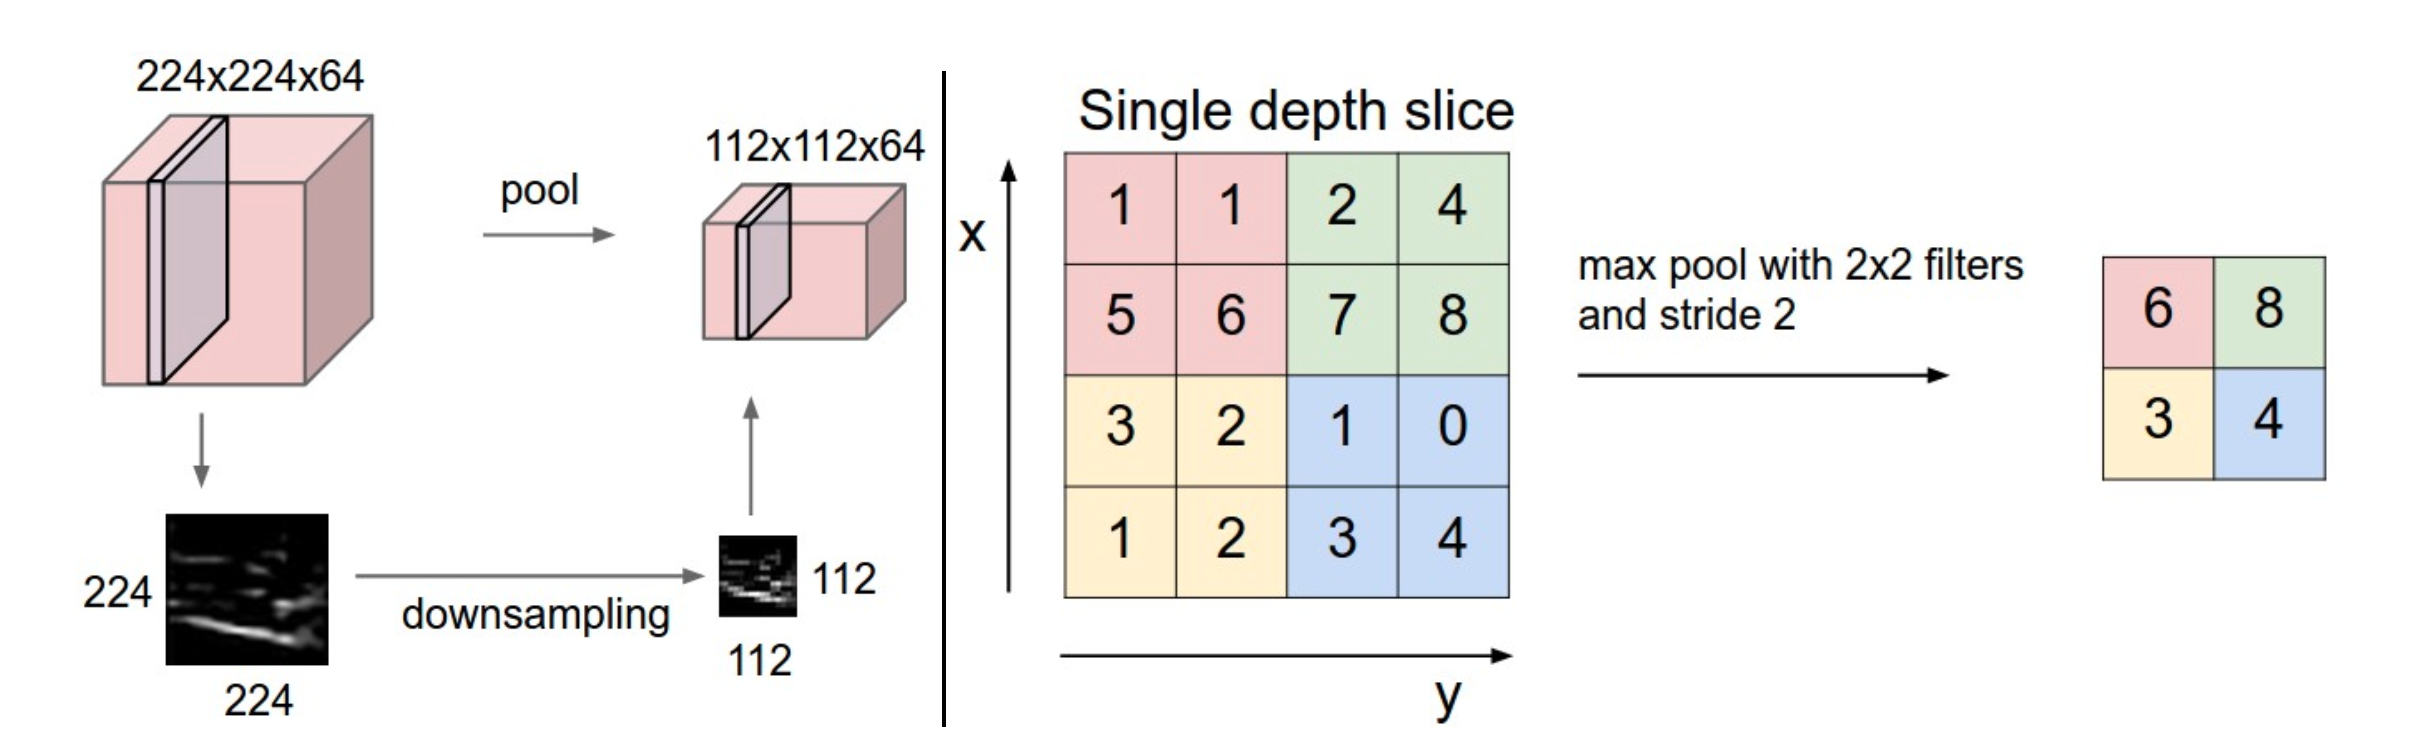
\includegraphics[scale=0.35]{chapter3/MaxPooling}
  \label{fig:MaxPooling}
\end{figure}

\quad

\subsection{AlexNet}

In 2012, a paper by Alex Krizhevsky started the new era of Convolutional Neural Networks, where CNN's were not only practically applicable to current visual problems like the ImageNet Large Scale Visual Recognition Challenge (ILSVRC) but beat the best results by a big margin~\cite{krizhevsky2012imagenet, imagenet}. The architecture by Alex Krizhevsky, a 5-layer CNN, achieved 15.3\% top-5 error rate and was named AlexNet after its creator. The next best result achieved a top-5 error rate of 26.2\% with versions of Fisher Vectors (FV) and Graphical Gaussian Vectors (GGV) after going through a feature extraction process with SIFT, CSIFT, LBP and GIST. Since then the winners of all subsequent ILSVRC challenges applied successfully a deep learning approach. \\

AlexNet uses eight learned layers of which five are convolutional, and three are fully-connected layers. After the convolutions, ReLU's are used for the activation function since they train several times faster than equivalent architectures trained with tanh or sigmoid functions. The last fully-connected layer is fed to a 1000-way softmax function that produces a distribution over all the 1000 classes giving the probability of a certain class to be contained in the image. For the input layer, the images are first resized to 256x256 pixels and then crops of size 227x227x3 are used as inputs into the model. 96 kernels of size 11x11x3 with a stride of 4 pixels are then applied on the input image leading to an output volume of 55x55x96. In the original paper, the filters were split across two GPU's but since the GPU's have increased their capacity and performance since 2012 hugely, this splitting is not applied on the current AlexNet architecture in this thesis. The formula for calculating the new output volumes is the following: \\

\[ O = {\frac{(W - F + 2P)}{S}} + 1 \] \\

with O standing for the output dimension (length of the width or height), W standing for the input length, F for the filter size, P for padding and S for stride. Max pooling is done after the first, second and fifth convolutions. Instead of going with the regular 2x2 pooling that halves the width and length dimensions of the input volume, AlexNet applies a 3x3 pooling with stride 2. They argue that it helps in reducing overfitting and leads to slightly better accuracies. The architecture can be seen in Figure~\ref{fig:AlexNet}. \\

\begin{figure}[!h]
  \centering
  \caption{The original architecture as proposed by Alex Krizhevsky with the distribution of the model and filter over two GPU's~\cite{krizhevsky2012imagenet}.}
  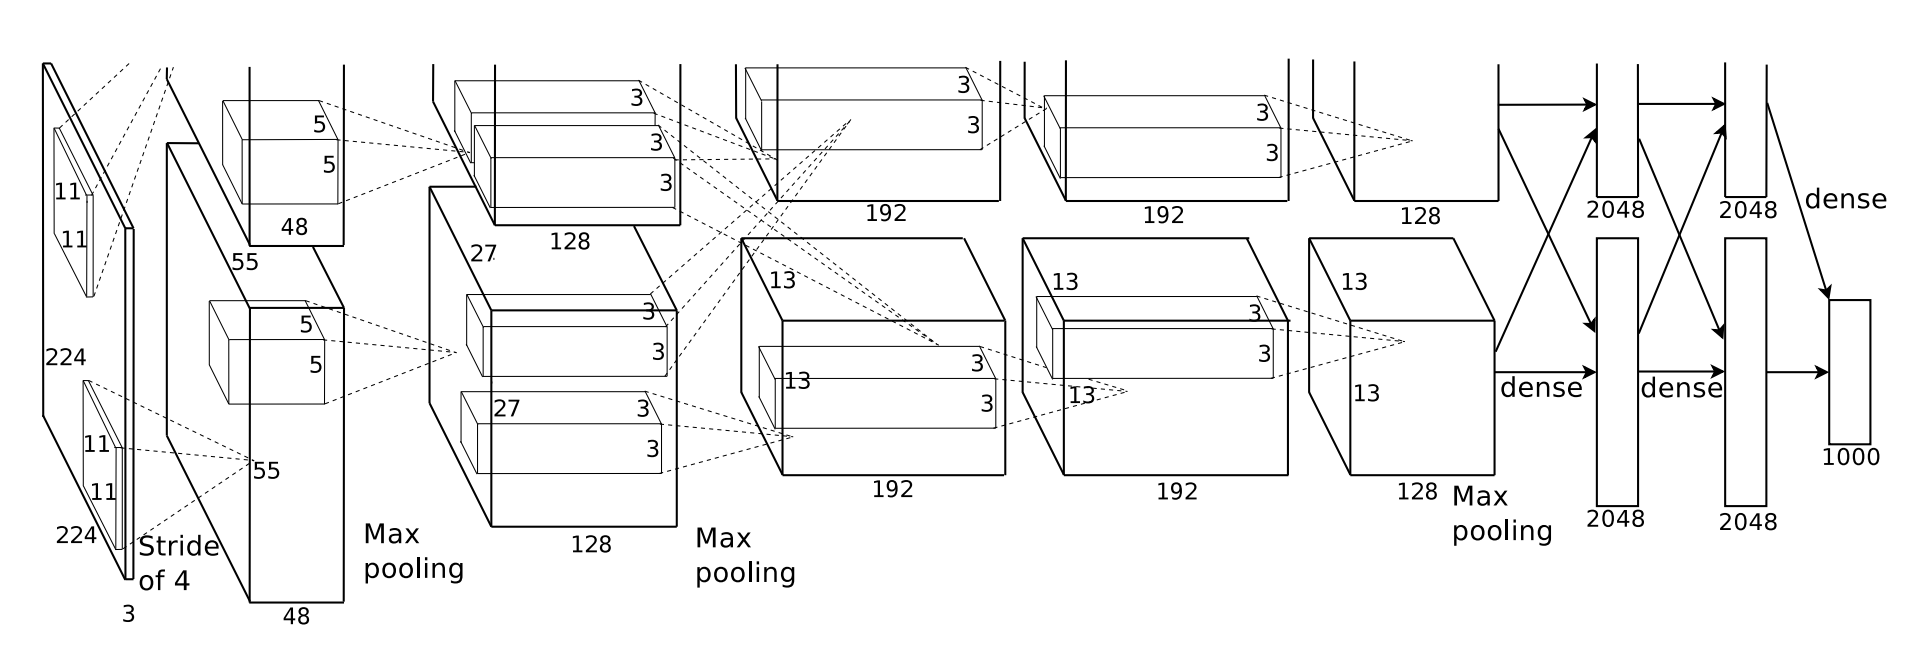
\includegraphics[scale=0.45]{chapter3/AlexNet}
  \label{fig:AlexNet}
\end{figure}

\quad

The horizontal separation of the architecture comes from the need to distribute the model and the filters over two GPU's. Unfortunately, the image was already cropped that way in the original paper of Alex Krizhevsky.

Although the architecture itself is very small compared to the later architectures, it still has over 60 million parameters to learn. These parameters are mostly located in the first and second fully connected layers. Learning so many parameters for classifying only 1000 objects might lead to overfitting of the training data. For the ILSVRC competition, two methods have been used. Heavy data augmentation using label-preserving transformations (increase images by factor 2048) and dropout in which certain hidden units are dropped for the current forward pass with some probability (often 0.5). \\

The winner of the ILSVRC 2013 was ZFNet which basically is the AlexNet architecture with very small alterations~\cite{zeiler2014visualizing}. Although the alterations are small they were very guided in their development through visualization techniques. Zeiler and Fergus visualized the layers and filters and deduced clear and specific improvements on AlexNet.\\


\subsection{VGG}

The 1st runner up winner of the ILSVRC 2014 was Karen Simonyan and Andrew Zisserman with their architecture named VGG~\cite{simonyan2014very}. Instead of further trying to fine-tune AlexNet they explicitly wanted to explore how the depth of an architecture plays out on accuracy and generalizability. For that reason, they used only 3x3 convolutions with a padding of 1 pixel and stride of 1 pixel as well followed by a ReLU activation function. Therefore the input volume from layer to layer stays the same while the number of filter increase after each max-pooling layer. If the spatial resolution needs to be reduced, max-pooling is applied with a 2x2 window and a stride of 2. This allowed Simonyan et al. to push the depth of the network to 16-19 layers. In the end, there are again 3 fully-connected layers as in AlexNet. The first two have 4096 hidden units and the third performs a softmax on the 1000 classes of ImageNet dataset. Figure~\ref{fig:vgg16} shows the original VGG16 architecture.\\


\begin{figure}[!h]
  \centering
  \caption{VGG16 architecture with 13 convolutional layers and three fully-connected layers at the end~\cite{ferguson2017automatic}.}
  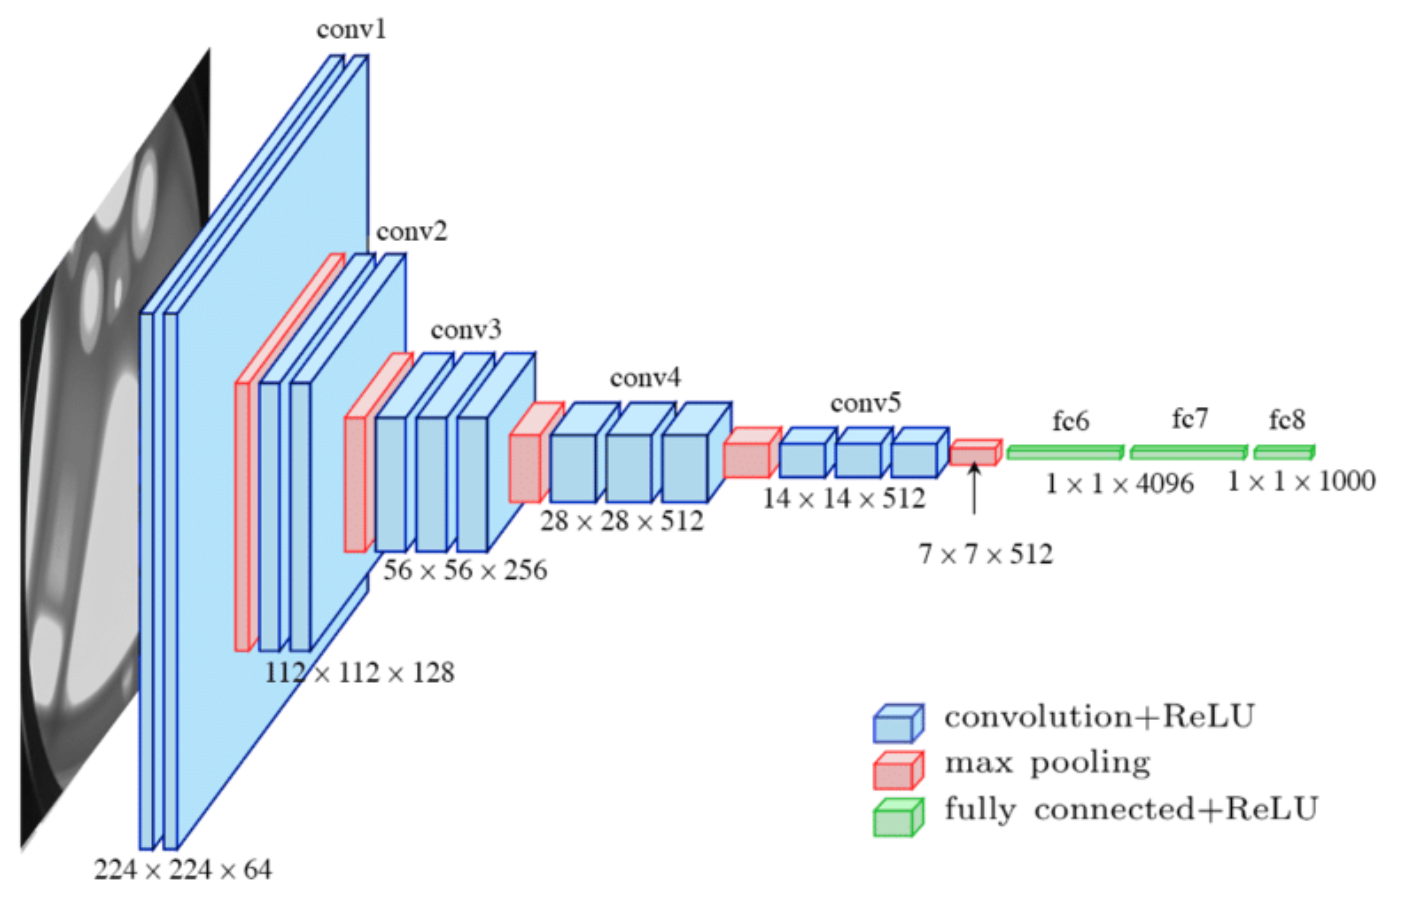
\includegraphics[scale=0.35]{chapter3/VGG16}
  \label{fig:vgg16}
\end{figure}

\quad

One of the bigger issues with the VGG architectures is their huge size in parameters, which ranges from 133 million parameters for the smaller VGG11 architecture to 144 million parameters for the bigger VGG19. This is a problem since it can be difficult to handle so many parameters and training takes much longer. The last three fully-connected layers contribute the large part of the parameters with the convolutional layers playing a minor role. Because VGG is very uniform with its 1 type of convolution and easy to understand, it enjoyed large acceptance with the community and was often used regardless of its size. Figure~\ref{fig:parameters} shows how different architectures perform relative to their size in parameters.


\begin{figure}[!h]
  \centering
  \caption{Performance of different architectures relative to their number of operations needed for one forward pass. The number of operations is proportional to the number of parameters used by the architecture~\cite{canziani2016analysis}.}
  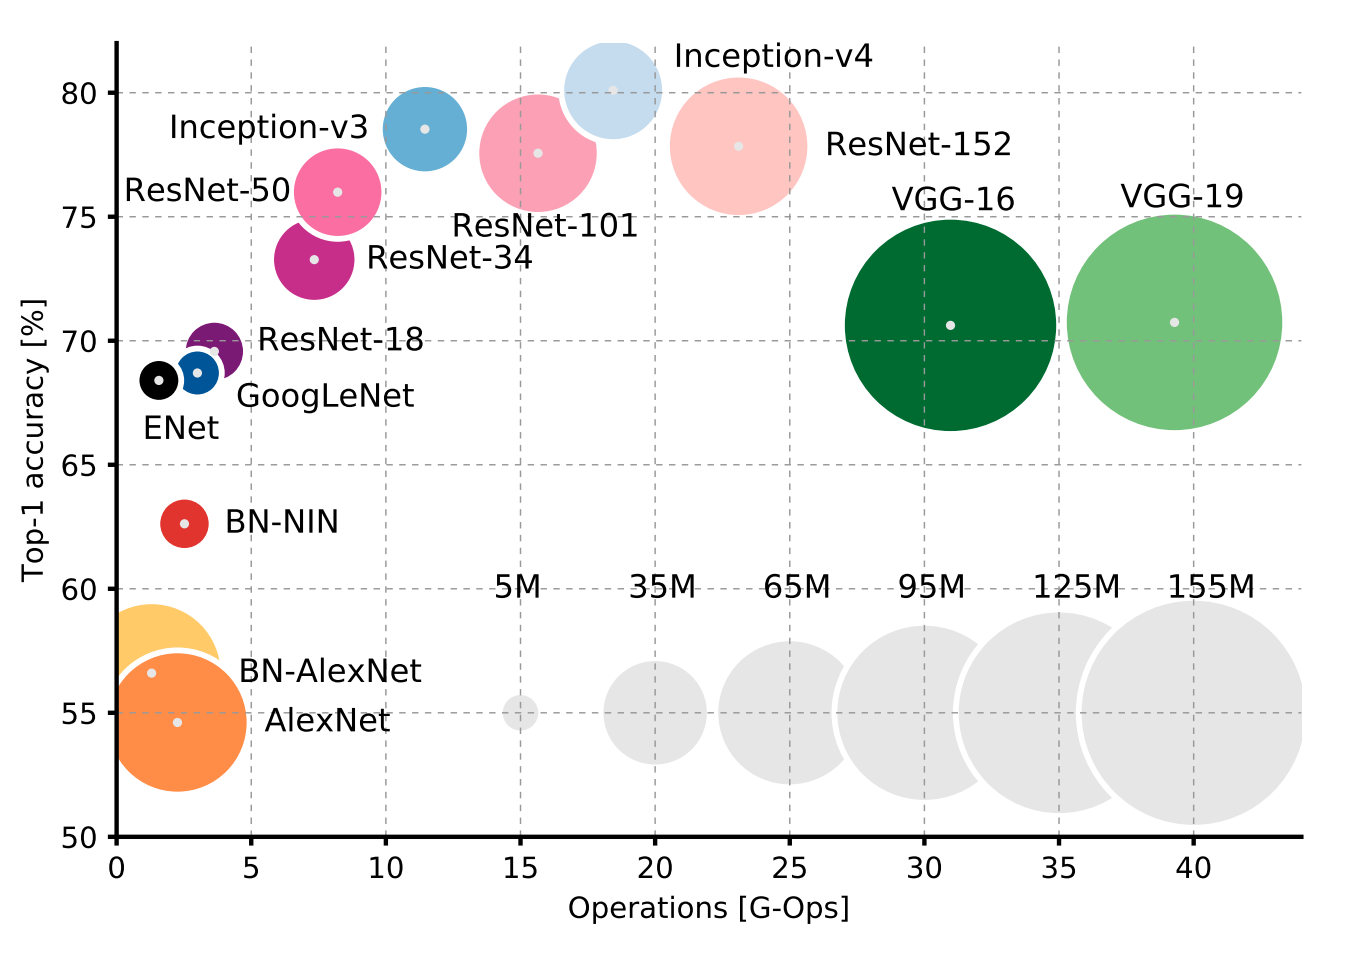
\includegraphics[scale=0.35]{chapter3/parameters}
  \label{fig:parameters}
\end{figure}


A slight positive correlation can be seen between the size of the network and its performance. VGG architectures are an exception. Although they performed really well in their time, they underperform when the network size is taken into consideration. All in all it cannot be said that more parameters  lead to better architectures. The following architectures (Inception, ResNet and Densenet) show how less parameters but better architectures can surpass human level performance.\\


\subsection{Inception}

The winner of the ILSVRC 2014 image classification was Szegedy et al. with their GoogleLeNet architecture~\cite{szegedy2015going}. Their network is quite different from the previous networks winning the ILSVRC competitions and applied 1 by 1 convolutions and global average pooling, both methods inspired from the "Network in Network" paper in 2013~\cite{lin2013network}. Another technique added to the architecture is the Inception module, which has convolutions of different sizes for the same input volume and stacking the results all on top of each other and into the output volume. \\

The 1x1 convolution is used to reduce the dimension along the length axis. E.g. in VGG with every max pooling layer the spatial dimensions got reduced by half but the depth of the volume got deeper with every additional max pooling layer, adding more filters to the computation. With a 1 by 1 convolution, the spatial dimensions are untouched but the length will be recast into the length of number of filters. Also, the computational effort gets reduced drastically with this method. In Figure~\ref{fig:InceptionRegularConv} a regular 5x5 convolution is performed on the input volume of 14x14x480 with 48 filter leading to an output volume of 14x14x48. Computationally that is very expensive with roughly 113 million single operations ( (14x14x48) x (5x5x480) = 9'408 x 12'000 = 112'896'000 ).\\


\begin{figure}[!h]
  \centering
  \caption{5x5 convolution is used with only 48 filters reducing the spatial dimensions and also the length of the volume~\cite{ReviewGoogleLeNetv1}.}
  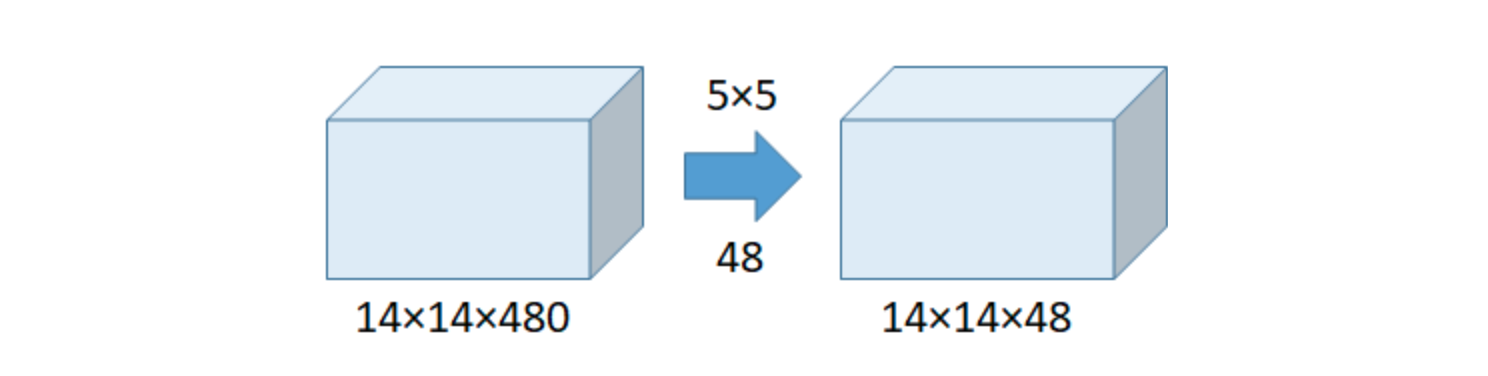
\includegraphics[scale=0.4]{chapter3/InceptionRegularConv}
  \label{fig:InceptionRegularConv}
\end{figure}

\quad

Adding a 1x1 convolution adds an additional step to the whole transformation but both steps are computationally very efficient. The first step is to convolve the input volume with 1x1 filters. In our example with 16 filters leading to the following computations: (14x14x16) x (1x1x480) = 3'136 x 480 = 1'505'280. Adding the second 5x5 convolution to it leads to (14x14x48) x (5x5x16) = 9'408 x 400 = 3'763'200. Adding the total computations of both convolutions together we get approximately 5.3 million operations compared to 112.9 million computations when not using dimensionality reduction. This is a huge gain in computational efficiency.\\


\begin{figure}[!h]
  \centering
  \caption{First a 1x1 convolution is performed in order to reduce the length of the volume leaving the spatial dimensions as is. In the next step, a 5x5 convolution, is performed with 48 filters~\cite{ReviewGoogleLeNetv1}.}
  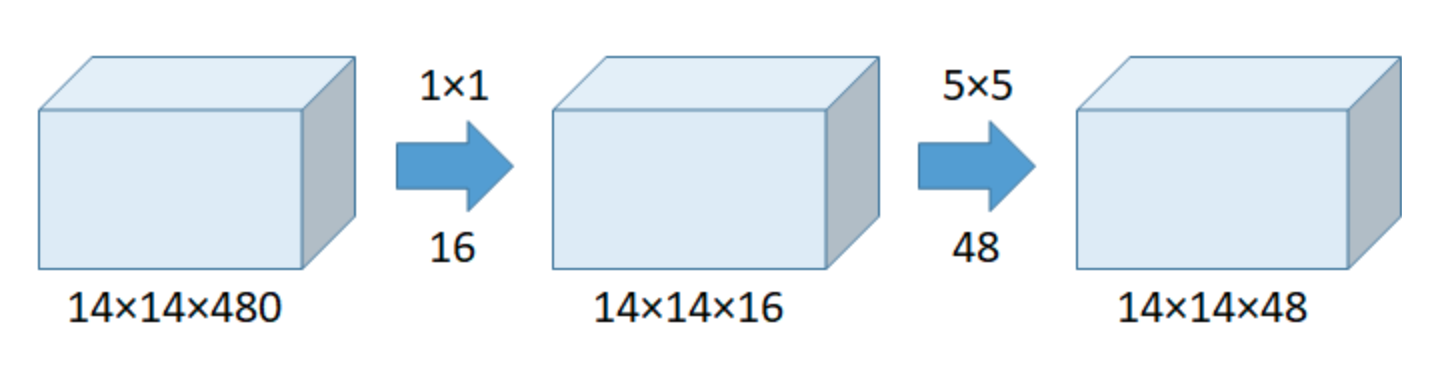
\includegraphics[scale=0.4]{chapter3/InceptionOneByOne}
  \label{fig:parameters}
\end{figure}

\quad

This technique reduces the model size without losing important information. It has been shown that the reduced number of parameters mitigated the problem of overfitting to the data and therefore lead to better results. 

An Inception module combines different convolutions together and stacks their output on top of each other. Table~\ref{fig:InceptionModuleNaiv} shows a naive Inception module without prior dimensionality reduction that would lead to a huge amount of computations needed. \\


\begin{figure}[!h]
  \centering
  \caption{Naive Inception module using different convolution filters and stacking the output on top of each oher. Computationally very expensive~\cite{ReviewGoogleLeNetv1}.}
  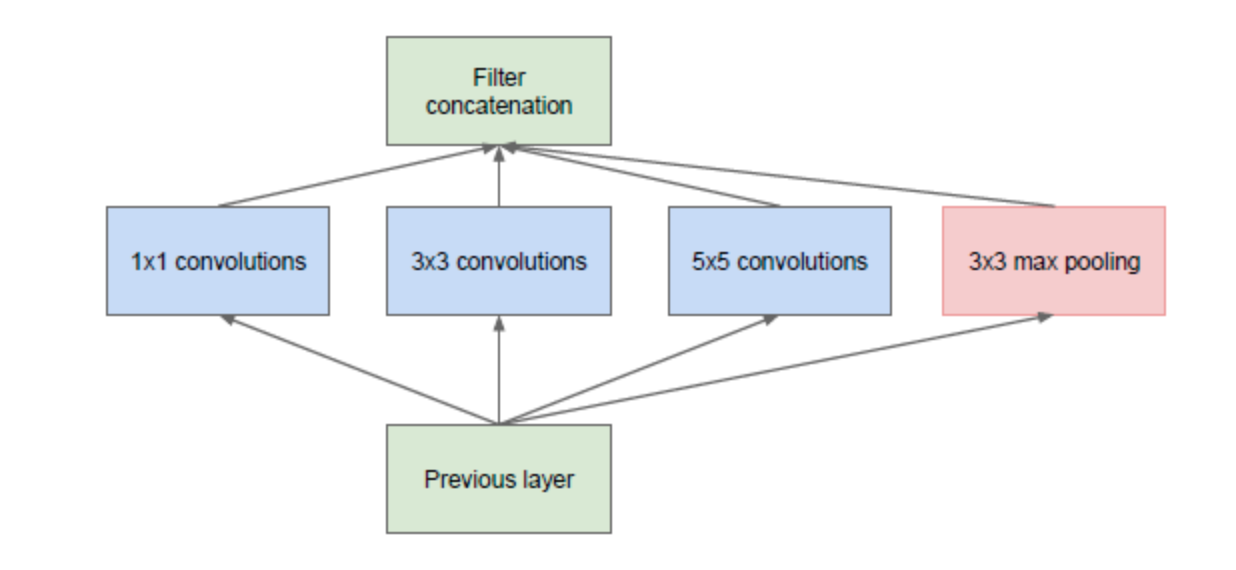
\includegraphics[scale=0.45]{chapter3/InceptionModuleNaiv}
  \label{fig:InceptionModuleNaiv}
\end{figure}

\quad

In Table~\ref{fig:InceptionModule} the Inception module is shown as it is used in the Inception network presented in~\cite{szegedy2015going} leading to a much more efficient implementation. Prior to the different convolutions, a 1x1 filter is applied to the input volume to reduce the size before the heavy lifting is done. With max-pooling it is the other way around. Max pooling reduces the size without any computational overhead and is therefore performed before the 1 by 1 convolution which still requires some amount of computation.\\


\begin{figure}[!h]
  \centering
  \caption{Inception module with 1x1 filters added before doing the different convolutions in order to reduce computation~\cite{ReviewGoogleLeNetv1}.}
  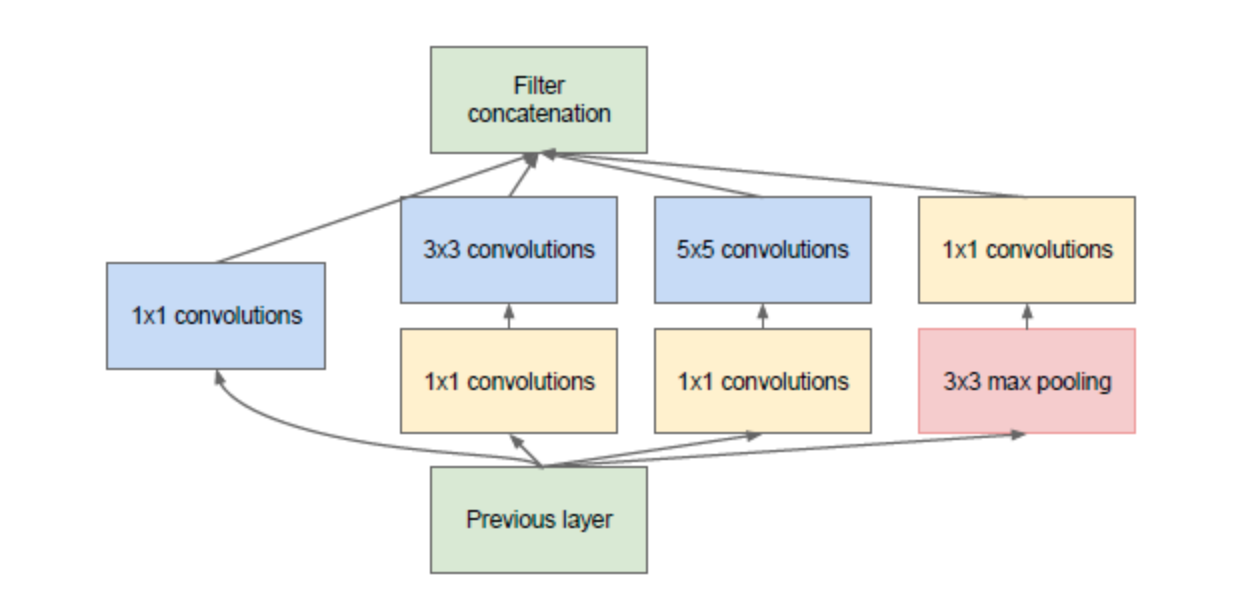
\includegraphics[scale=0.45]{chapter3/InceptionModule}
  \label{fig:InceptionModule}
\end{figure}

\quad

The third improvement of GoogLeNet is the global average pooling at the end instead of having three fully-connected layers. AlexNet, ZFNet and VGG all used the common practice to have three fully-connected layers with the last layer being a softmax function. These three last layers made up the bulk of all the parameters used increasing the complexity of the models. Figure~\ref{fig:GlobalAveragePooling} shows on the left side a common transition from a layer with many filters (1024 in that case) to the next layer. 1024 filters with dimension 7x7 make 50'176 parameters. If they are fully connected with the next layer which consists of 1024 units it results in 50'176 x 1024 = 51'380'224 weights! With global average pooling as seen on the right side of Figure~\ref{fig:GlobalAveragePooling} the 7x7 filters get averaged into a 1x1 scalar of which 1024 are computed. With averaging the values into one new value no new weights are introduced. Not only is that method much more efficient and reduces the overall complexity but it also can help to reduce the problem of overfitting as mentioned in the Network in Network paper \cite{lin2013network}.\\


\begin{figure}[!h]
  \centering
  \caption{On the left side a commonly used fully connected layer is shown. On the right side a global pooling layer is shown as introduced in GoogLeNet~\cite{ReviewGoogleLeNetv1}.}
  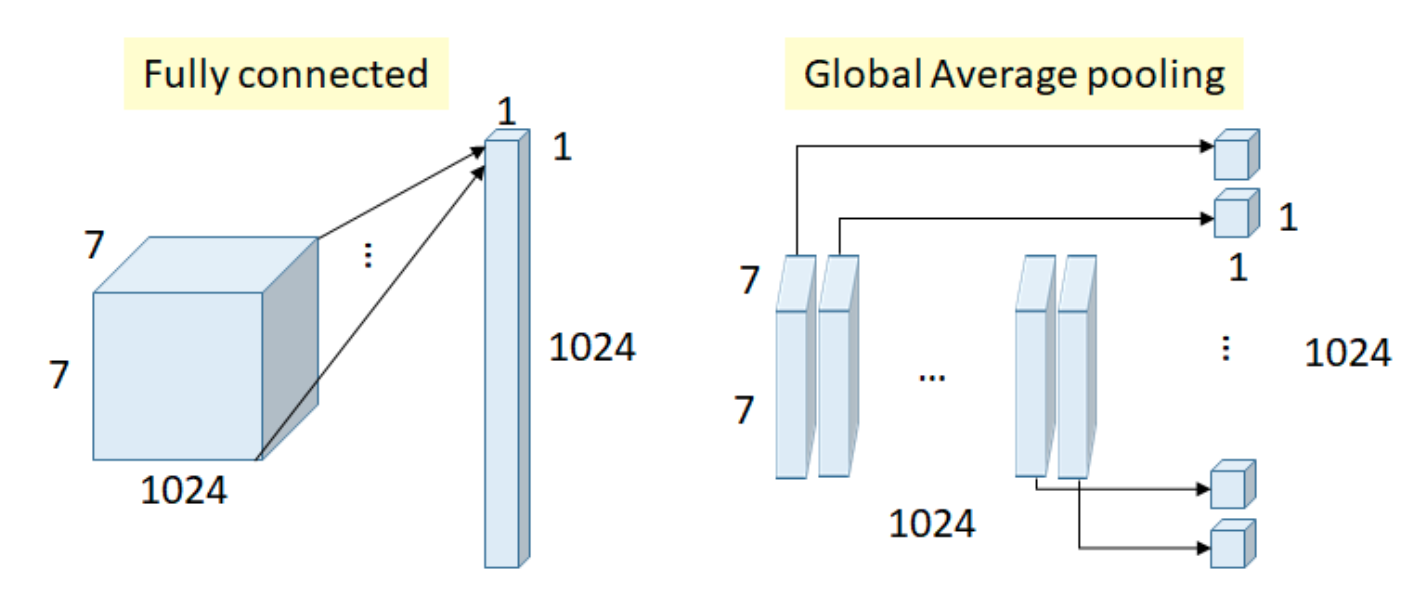
\includegraphics[scale=0.45]{chapter3/GlobalAveragePooling}
  \label{fig:GlobalAveragePooling}
\end{figure}

\quad

Inception v3 was the first runner up for image classification in ILSVRC 2015 and came with some refinements over the first version described above~\cite{szegedy2016rethinking}. Inception v3 is also used in the implementation and evaluation part of this thesis. The first refinement was adding batch normalization~\cite{ioffe2015batch}. The second refinement was adding factorizing convolutions to reduce even more parameters without decreasing the architectures efficiency leading to the Inception v3 model. Table~\ref{fig:factorization} shows how a 5x5 filter with 25 parameters can be realized with two 3x3 filters with 9 parameters each summing up to 18 parameters which is a reduction by 28\%. \\


\begin{figure}[!h]
\centering
\caption{Factorizational Convolution reduces parameters by using smaller filters.}
\subfigure{
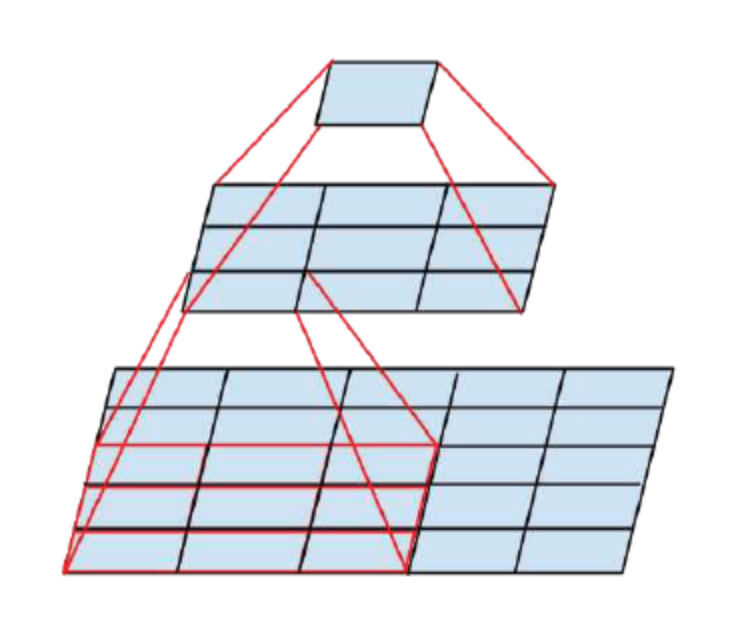
\includegraphics[width=.4\textwidth]{chapter3/FactorizationA}
}
\subfigure{
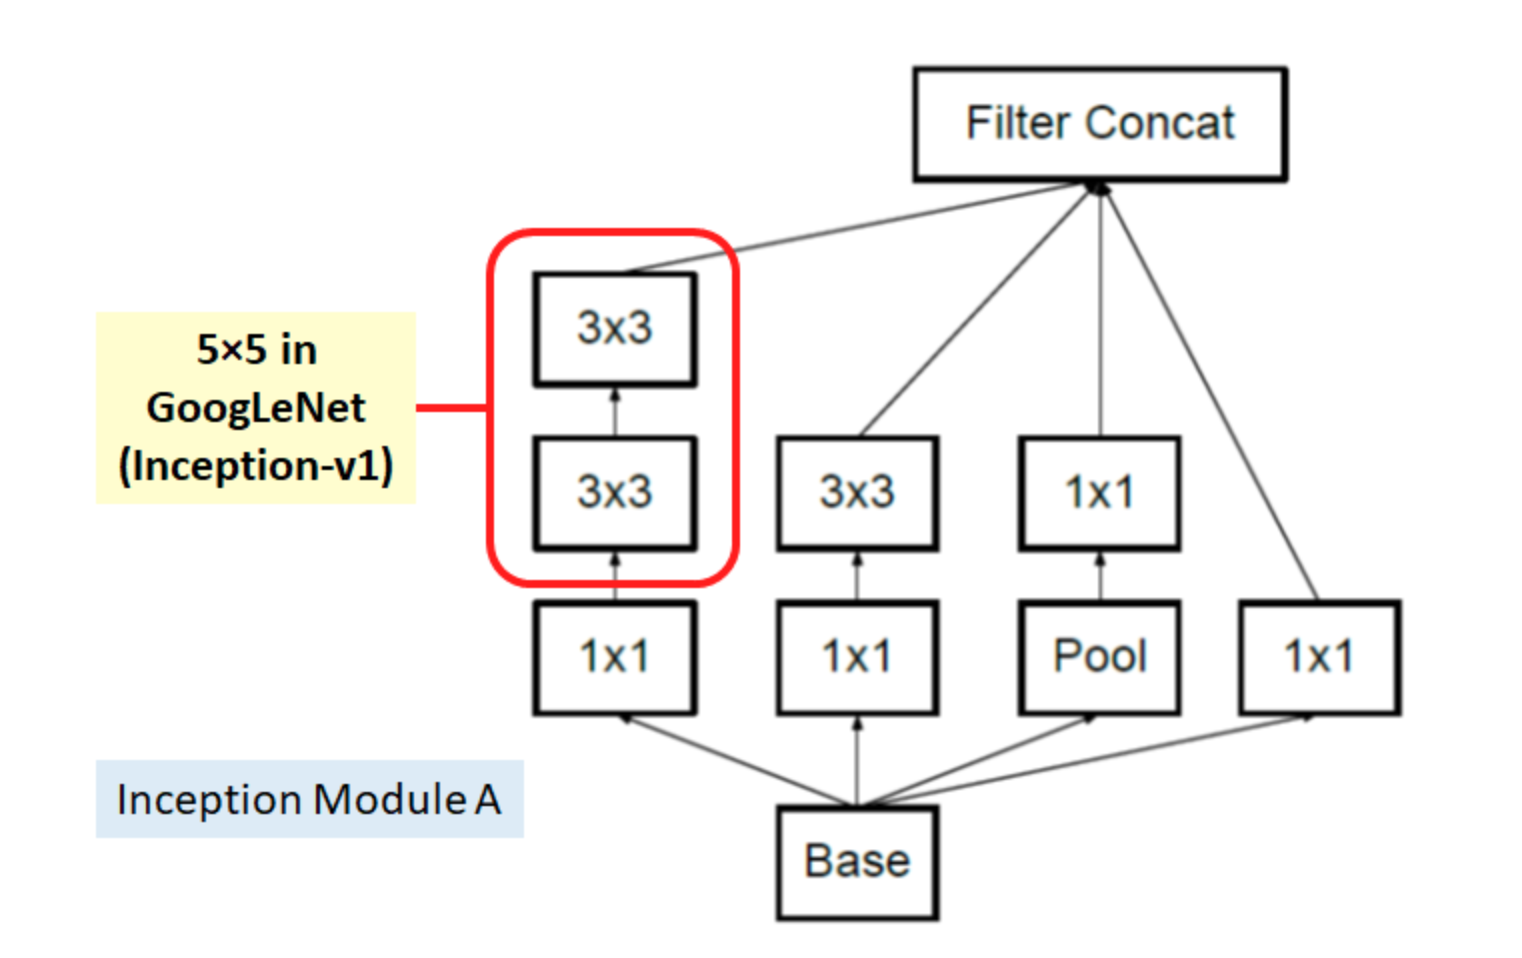
\includegraphics[width=.5\textwidth]{chapter3/FactorizationB}
}
\label{fig:factorization}
\end{figure}

\quad

There are additional asymmetric convolutions where a 3x3 filter can be realized with two filters of the following sizes: 1x3 and 3x1. This also reduces the overall parameters used. Another minor modifications are done to the auxiliary classifier and grid size reduction~\cite{szegedy2016rethinking}.\\



\subsection{ResNet}

The winner of the ILSVRC 2015 were Kaiming He et al. with their very deep architectures applying residual connections~\cite{he2016deep, he2016identity}. Their architecture was named ResNet and was specifically created with depth in mind. Zeiler et al. have shown how deep networks are naturally able to integrate low/mid/high-level features and that depth seems to enrich these features leading to better performance~\cite{zeiler2014visualizing}. Leading results in the ImageNet challenge like the aforementioned VGG~\cite{simonyan2014very} and LeNet~\cite{szegedy2015going} all exploit deeper architectures. There are a few obstacles of going simply deeper with the current models except computational power. One issue arises from the vanishing/exploding gradient which happens during backpropagation~\cite{glorot2010understanding}. The weights get updated during learning by multiplying the weights with the gradient from the partial derivatives of the loss function. This leads to the chain rule being applied as many times as layers are present in the network. If the gradient is some small number below 1 it gets multiplied many times over and over, leading to a vanishing value that makes is very difficult to train the layers in the beginning of the network. The same holds true if the gradients are big or above 1. Then they explode by getting bigger and bigger with every layer. But even if the vanishing/exploding gradient can be mitigated with better weight initialization and intermediate normalization layers~\cite{ioffe2015batch}, the degradation problem prohibits the learning of deeper networks, where the accuracy gets saturated and starts degrading with more layers~\cite{he2016deep} regardless of the vanishing/exploding gradient issue. This observed degradation is also not caused by overfitting to the training data~\cite{he2015convolutional, srivastava2015highway}.\\

ResNet architectures address this degradation problem by introducing residual mappings which also mitigate the vanishing/exploding gradient problem. These residual mappings are easier to optimize than the unreferenced mappings. If for example, it would be optimal to apply the identity mapping, pushing the residual mapping to zero is much easier for the network than fit an identity mapping by a stack of nonlinear layers. Figure~\ref{fig:ResidualBlock} shows such a residual block.\\


\begin{figure}[!h]
  \centering
  \caption{A building block for residual learning~\cite{he2016deep}.}
  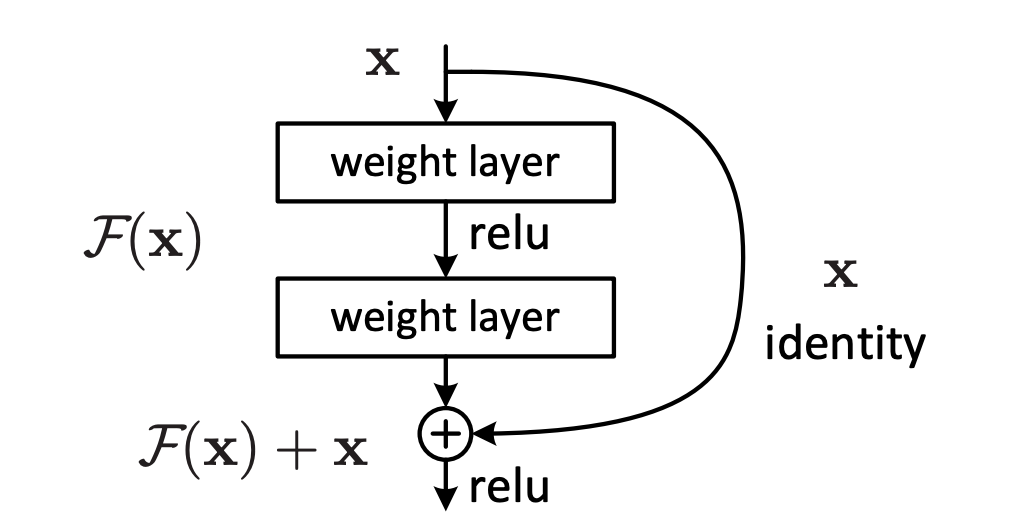
\includegraphics[scale=0.35]{chapter3/ResidualBlock}
  \label{fig:ResidualBlock}
\end{figure}

\quad

As seen in Figure~\ref{fig:ResNet} an activation layer is skipped over and the output from the previous layer ($L^{i-1}$) is simply forwarded to two layers ($L^{i+1}$) jumping over one layer ($L^{i}$). If the identity mapping were the optimal mapping, the architecture is now able to drive F(x) to zero making the addition in the second layer an identity mapping. That is much easier than trying to find some F(x) mappings that approximate the identity mapping. Therefore, depth does not automatically degrade the performance of the architecture, since these skip connections omit further optimization that doesn't work.\\


\begin{figure}[!h]
  \centering
  \caption{Comparison of the VGG-19 architecture with a 34-layer plain model and its residual counterpart. Notice that only the VGG architecture has 3 fully-connected layers. By omitting these 3 fully-connected layers in the ResNet architecture the overall complexity is drastically reduced~\cite{he2016deep}.}
  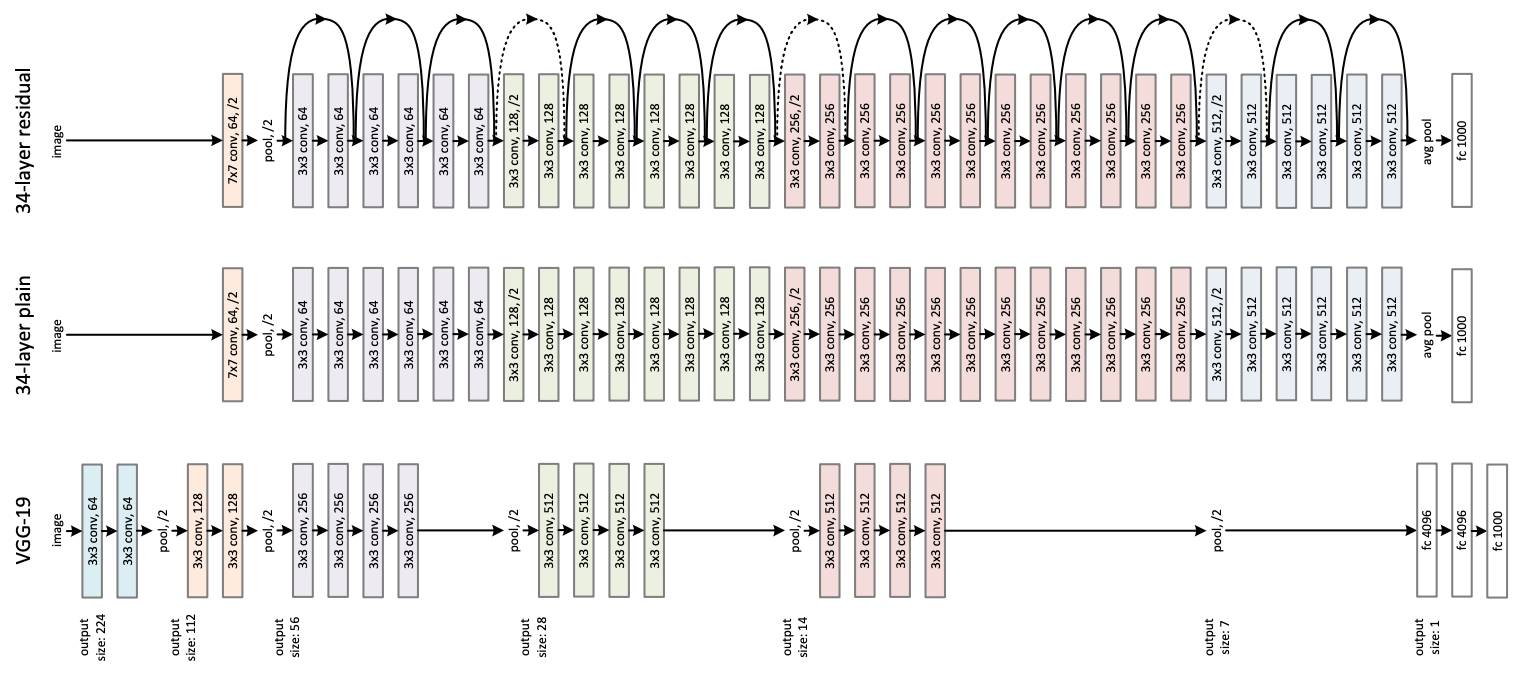
\includegraphics[scale=0.35]{chapter3/ResNet}
  \label{fig:ResNet}
\end{figure}

\quad

\subsection{Densenet}

A common problem of deep networks is the passing of information from one layer to the next layer in a feed-forward manner. A very deep network needs to pass the input through many layers, which can "wash out" by the time it reaches the softmax function or the global average pooling layers. The same holds true for the gradient being passed back to the beginning of the network, as explained in the previous subchapter on the ResNet architecture. The Dense Convolutional Network (DenseNet) solved this problem with densely connecting all layers with each other that reside in a dense block~\cite{huang2017densely}. A dense block
consists of several layers made up of batch normalization, activation function (ReLU) and a SAME convolution that retains the spatial size of the input. Such a dense block is shown in Figure~\ref{fig:DenseBlock}. All the layers within the dense block are fully connected with each other in order to implement its own skip connection functionality. The short connections are only possible within a dense block since all the filters are stacked on top of each other and forwarded to every subsequent layer.\\


\begin{figure}[!h]
  \centering
  \caption{Shown is one dense block of a DenseNet architecture. In the original paper 4 dense blocks were used to create DenseNet~\cite{huang2017densely}.}
  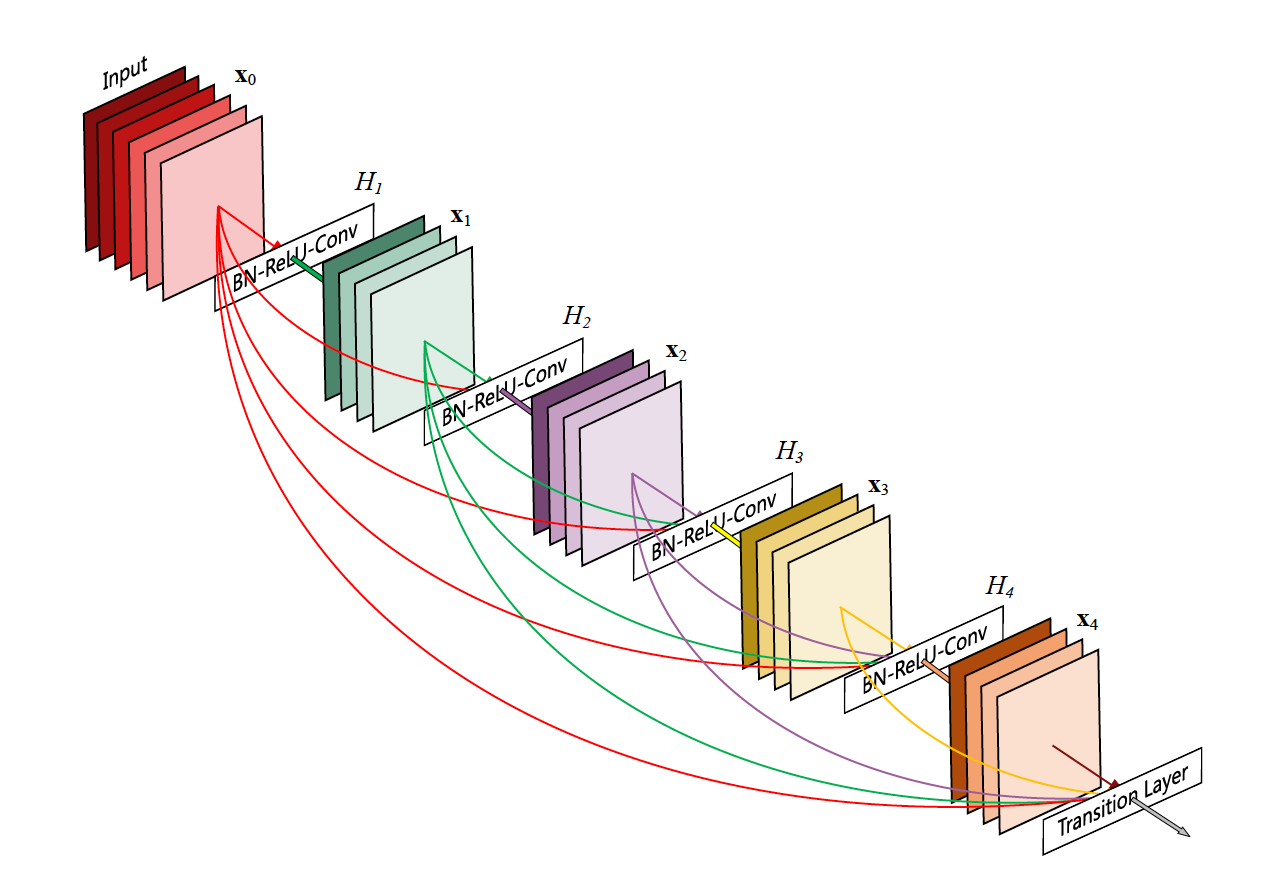
\includegraphics[scale=0.45]{chapter3/DenseBlock}
  \label{fig:DenseBlock}
\end{figure}

\quad

After each dense block, a 1x1 convolution is used to reduce the number of filters. After this so-called bottleneck layer, a 2x2 average pooling layer, is applied to reduce the spatial dimensions of the input volume as shown in Figure~\ref{fig:DenseNet}.\\


\begin{figure}[!h]
  \centering
  \caption{This Figure shows how the isolated dense blocks are connected through convolution and pooling layers into a full DenseNet architecture~\cite{huang2017densely}.}
  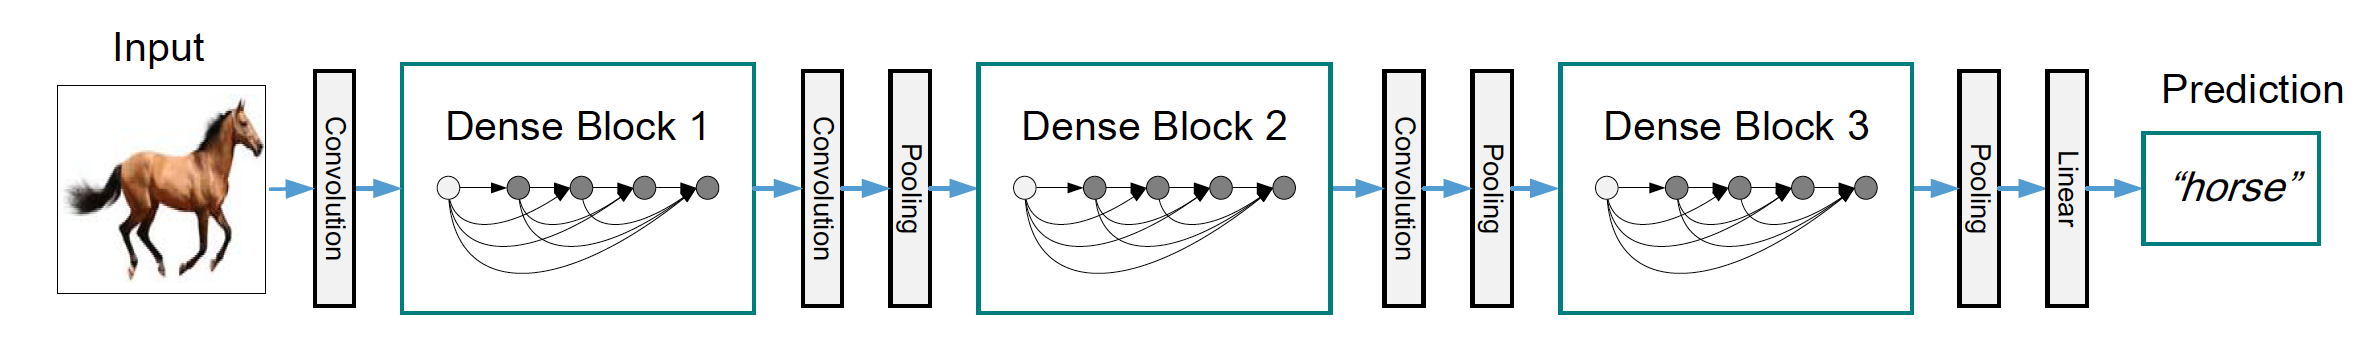
\includegraphics[scale=0.35]{chapter3/DenseNet}
  \label{fig:DenseNet}
\end{figure}

\quad

DenseNet introduces several new parameters like the growth rate k which limits the growth of the network and thus limiting the width of the network. A growth rate of 12 means that each layer may only add another 12 filters to the existing filters prior to this layer. Another interesting parameter is the compression which improves the compactness of the model by defining how much of the feature-maps get transitioned to the next dense block. The compression value is between 0 and 1 without including the value 0.\\


\section{Deep learning frameworks}

There are two main deep learning frameworks that can readily be used. Tensorflow~\cite{tensorflow} which was originally developed by researchers and engineers at Google Brain and is based on Theano. The other deep learning framework is PyTorch~\cite{pytorch} that was built by researchers at Facebook. They are both open source and free to use, but the flavor is quite different. While TensorFlow uses static computational graphs that need to be built prior to compilation and run in their run engine, PyTorch uses dynamic computational graphs that can be rather interpreted than compiled. Programming in PyTorch is much more pythonic whereas in TensorFlow the user needs first to get used to the way things are handled in TensorFlow, which at times can be quite different, like building the whole computational graph in advance, using placeholders for all weights and variables, then creating a session in which the graph can be executed. Debugging in TensorFlow is more difficult since it needs at least two different debuggers to be used. One for the tensors and their values, and one for the python code itself. That makes it much less intuitive to simply debug the underlying code while keeping track of all tensors. In PyTorch, the native debugger may be used for the whole codebase, including all the variables and weights. Data parallelism is much easier to use in PyTorch since the distribution of the code and data onto all the GPU's happens automatically. Whereas in TensorFlow much more manual work and careful thought need to be applied to achieve the same behavior. Since PyTorch is one big framework it gives more the feeling of working with one framework that uses a very pythonic way to handle things. TensorFlow, on the other hand, is more like an aggregation of many libraries that work together to achieve a common goal. Although that was the case in early 2018 things are changing very fast for these frameworks. Tensorflow was much better for production environments but with PyTorch version 1.0 this advantage is closing fast~\cite{pytorchOnePointZero}. Table~\ref{tbl:DeepLearningFrameworks} summarizes the different qualities of both frameworks at the start of the master thesis in late summer 2018. \\

\begin{table}[t] \centering
\ra{1.3}
\caption{Different qualities of the deep learning frameworks: PyTorch and TensorFlow}
\begin{tabular}{@{}rrr@{}}
\toprule & PyTorch & TensorFlow \\
\midrule
Open-source									& + & + \\
Dynamic Computational Graph			& + & -  \\
Static Computational Graph				& - & +  \\
Easy Learning Curve							& + & -  \\
Fast developing of new Models			& + & -  \\
Production Environment					& - & + \\
Developer Community						& + & + \\
Native Visualization							& - & +  \\
Debugging										& + & -  \\
Data-Parallelisme								& + & -  \\
Framework-Feeling							& + & -  \\
Library-Aggregation							& - & +  \\

\bottomrule
\end{tabular}
\label{tbl:DeepLearningFrameworks}
\end{table}

\quad

There are some higher level frameworks like Keras~\cite{keras} and DeepDIVA~\cite{deepdiva} that enable many more features and faster development. Keras is built on top of TensorFlow and has many models pre-implemented. It enables the developer to very quickly start modeling a problem or apply already present architectures to new data. It does not allow the same flexibility as TensorFlow but if a new architecture needs to be designed from scratch it is done in TensorFlow than made available on Keras as to use on different datasets or different tasks. A possible counterpart for Keras is DeepDIVA that was developed at the University of Fribourg by the DIVA group. It has been built to be used on top of PyTorch and also provides pre-implemented architectures or allows to include them in a straight-forward manner. It tackles some of the disadvantages of PyTorch versus Tensorflow like including TensorBoard Visualization to PyTorch. Development in DeepDIVA is also very pythonic and does not actually change at all since it is very tightly integrated into the PyTorch framework. Creating new architectures or altering existing ones is straight forward.\\


\section{Tools}

Apart from PyTorch and DeepDIVA there is need for some other tools as well like programming IDE's, text and math editors and version control systems. Additionally, the obtained results and data need to be visualized and some optimization tools might be better than others.\\


\subsection{Visualization}

With CNN's it is very difficult to really know what they have learned. There are several examples where an architecture performed exceptionally well on the test set but later it was found out that it did not really recognize the object itself but some other characteristics unrelated to the studied class. This is especially important when working with only a few classes. It is indeed very unsatisfactory from a scientific standpoint to use the accuracy alone to determine if an architecture is well suited for a problem or not. Even with other statistical parameters added, it still lacks a deeper understanding. There are several methods on how to study what a model really learns and to visualize it. Since this is still quite a young field of research, it is quite difficult to find good libraries that can be applied to the problem.The visual toolbox by Utku Ozbulak~\cite{viztoolbox} will be adapted and plugged into the DeepDIVA framework and hopefully produce good and conclusive visualizations. It remains unclear if applying this library to other architectures than AlexNet and VGG will work. From the insights gained, modifications to existing architectures might be considered. \\


\subsection{SigOpt}

With all deep learning approaches it is vital to fine tune the hyper parameters like learning rate, momentum and weight-decay to the architecture and problem at hand. Often considerable amount of time is invested into this process in order to reach the best possible accuracies and reach current state-of-the-art performance. Using gridsearch for optimizing the hyper parameters would require hundreds of separate runs to find good values while only checking the value range in a very sparse manner. For the first and second baseline gridsearch was applied for comparison reasons, but gridsearch has many downsides like not being able to densly search through the searchspace but only taking the predefined values along the range. Applying gridsearch on only 3 hyper parameters with 10 predefined values per hyper parameter leads to 1'000 separate runs which is not feasible. SigOpt~\cite{sigopt} is a company that specializes on hyper parameter optimization. They employ bayesian optimization which efficiently trades off exploration and exploitation of the pre-defined hyper parameters and their respective parameter space. Thus it moves quickly towards an optimal configuration that best optimizes the user's defined evaluation criterion. Common practice is to use 10 to 20 runs for each parameter which needs optimization~\cite{sigoptObservationBudget}. Bayesian optimization applies mainly methods from regression models and acquisition functions, that are used together to allow fast and guided configuration search~\cite{sigoptBayesian}. SigOpt generously provided a free academic account for the duration of this thesis and all architectures have been optimized with their product. \\


\subsection{PyCharm, GIT, R and Latex}

PyCharm~\cite{PyCharm} is an Integrated Development Environment (IDE) for the Python programming language and has many useful features on board like code completion, static code analysis and an own debugging environment. Being able to connect through SSH with a remote server allows to modify the remote code locally within PyCharm IDE and push all changes to the remote server on every save command. Remote debugging is also available with the professional license, which is free for students. Writing local scripts and integrating them with the existing PyTorch and DeepDIVA framework is easy and git~\cite{git2019} is implemented directly into PyCharm which makes it easy to do almost everything within the IDE itself.
For version control, forking the original repository and adding modifications to it, GitHub~\cite{GitHub} is used in combination with PyCharm and SourceTree~\cite{SourceTree} as a visual GUI.
Visualizing the obtained data was done with the statistical program R~\cite{statR} and RStudio~\cite{rstudio} and the python libraries matplotlib and seaborn. This thesis is written in Latex~\cite{latexProject2019}.\\


\section{Hardware}

The hardware used is provided by the Information and Communication Department of the HEIA-FR and consists of 4 Tesla K80 Graphics Cards with each 12GB of Memory and CUDA version 10.0. It is used on an Ubuntu 18.04 machine with 32 Intel(R) Xeon(R) CPU E5-2620 cores and 126 GB of RAM.\\


\section{Conclusion}

This chapter provided an analogy between biological neurons and artificial neurons in ANNs and cautioned from drawing too many conclusions from it. The abstraction might help to visualize and understand an artificial neuron but is oversimplified in most aspects. MLPs and their disadvantage of the exponential increase of parameters with every additional layer were discussed leading up to the convolutional neural network which solved this problem with small convolution filters that reduced the parameter size drastically and additionally encoded spatial information. The winners of ILSVRC were introduced one by one with AlexNet being the first CNN architecture to win the ILSVRC in 2012. All discussed architectures found their way into this thesis and will be compared against each other in many different configurations. \\

As for the framework, PyTorch with DeepDIVA have been chosen since they allow developing in a very pythonic way, have a native debugger that works for the code and the tensors equally well. Debugging capabilities are crucial for learning and developing new architectures. DeepDIVA has pre-defined architectures to start from and provides a TensorBoard implementation for visualizations. \\

For the visualization of the different layers of the network Utku Ozbulak's visualization toolbox~\cite{viztoolbox} was used. It is implemented in PyTorch and can be applied with some code adaptations to the AlexNet and VGG models. It has many different visualization modes to chose from and is quite extensive. It also provides a heat map visualization that shows which areas of the image contributed to classifying the image one way, or the other way.\\

Gridsearch and SigOpt were both used for hyper parameter optimization initially but for the more complex architectures only SigOpt was used since it allows for more fine-grained values and leads to better results within a smaller time frame. \\